\documentclass[12pt]{article}

\usepackage[]{graphicx}
\usepackage[]{color}
\usepackage{alltt}

\newcommand{\mytitle}{Functional ANOVA Decomposition}
\newcommand{\myname}{Juliet Fleischer}
\newcommand{\mysupervisor}{Prof. Dr. Thomas Nagler}

\usepackage[a4paper, width = 160mm, top = 35mm, bottom = 30mm, 
bindingoffset = 0mm]{geometry}
\usepackage{setspace}
\onehalfspacing
\usepackage[utf8]{inputenc}
\usepackage{amssymb}
\usepackage{amsmath}
\usepackage{adjustbox}
\usepackage{ragged2e}
\usepackage{xcolor}
\usepackage[round, comma]{natbib}
\usepackage{fancyhdr}
\usepackage{textcmds}
\usepackage{subcaption}
\usepackage{wrapfig}
\usepackage{tikz}
\usetikzlibrary{shapes, positioning}
\newcommand{\changefont}{%
    \fontsize{8}{11}\selectfont
}
\usepackage{amsthm}
\newtheorem{proposition}{Proposition}[section]
\newtheorem{definition}{Definition}[section]
\newtheorem{lemma}{Lemma}[section]
\newtheorem{theorem}{Theorem}[section]
\newtheorem{condition}{Condition}[section]
\newtheorem{example}{Example}[section]
\usepackage{hyperref}
\providecommand*{\definitionautorefname}{Definition}
\providecommand*{\propositionautorefname}{Proposition}
\providecommand*{\conditionautorefname}{Condition}
\providecommand*{\exampleautorefname}{Example}
\hypersetup{
  colorlinks = true,
  linkcolor = black,
  urlcolor = black,
  citecolor = black}
\pagestyle{fancy}
\fancyhead{}
\fancyhead[R]{\changefont{\mytitle}}
\fancyfoot{}
\fancyfoot[R]{\thepage}
\setlength{\headheight}{14.5pt}
\setlength{\parindent}{15pt} % default is usually 15pt
\setlength{\parskip}{0pt}    % no extra vertical space
\interfootnotelinepenalty = 10000

% ------------------------------------------------------------------------------
% MAIN -------------------------------------------------------------------------
% ------------------------------------------------------------------------------
\IfFileExists{upquote.sty}{\usepackage{upquote}}{}
\begin{document}

% FRONT PAGE -------------------------------------------------------------------
 
\begin{titlepage}
\begin{center}
    
\LARGE
Bachelor's Thesis
    
\vspace{0.5cm}
      
\rule{\textwidth}{1.5pt}
\LARGE
\textbf{\mytitle}
\rule{\textwidth}{1.5pt}
   
\vspace{0.5cm}
      
\large
Department of Statistics \\
Ludwig-Maximilians-Universität München 

\vfill

\Large
\textbf{\myname}

\vfill

\large
Munich, July 31\textsuperscript{th}, 2025
      
\vfill


\includegraphics[width = 0.4\textwidth]{sigillum.png}

\vfill

\normalsize
Submitted in partial fulfillment of the requirements for the degree of B. Sc.
\\

Supervised by \mysupervisor

\end{center}
\end{titlepage}

% CONTENTS ---------------------------------------------------------------------

\pagenumbering{Roman}
\newpage

\begin{abstract}

This article studies the functional ANOVA decomposition (fANOVA) in the context of model interpretability.
We begin by introducing the classical fANOVA, which assumes independent inputs, and illustrate its equivalence to the Hoeffding decomposition under zero-centered variables with an example. We then unify different notations under the concept of orthogonal projections and briefly present the variance decomposition. Next, we extend fANOVA to settings with dependent inputs, discussing two different formalizations and highlighting why one is more suitable for deriving an explicit solution in an exemplary decomposition, while the other remains primarily theoretical. Finally, we adopt an applied perspective, visualizing the decomposition of various functions and providing a conceptual overview of current estimation approaches.
\end{abstract}

\newpage

% Acknowledgements
\section*{Acknowledgements}

I would like to express my sincere gratitude to my supervisor, Prof.\ Dr.\ Thomas Nagler, whose guidance and support were essential to the success of this thesis. 
His expertise and constructive feedback not only shaped the direction of this work but also made the process of writing it both enjoyable and rewarding.
I am also thankful for the presence and encouragement of my friends during this period, which provided me with motivation and balance alongside my studies.
\newpage


\tableofcontents

%%%% if you would want to include material overview
%%%% use one of the following in addition
\newpage
\listoffigures
\newpage
% \listoftables
% \newpage

% CHAPTERS ---------------------------------------------------------------------

\pagenumbering{arabic}

\section{Introduction}\label{sec:intro}
% The mathematics of cooperation and attribution.

\subsection*{Questions}
\subsubsection*{Clarifying the connection between fANOVA, expected value, and projection \& bringing together different definitions}
When I start from \cite{muehlenstaedt2012} and basically go the way: \textit{fANOVA term $\rightarrow$ expected value $\rightarrow$ projection}, I arrive at the formulation where we first compute the projection and afterwards subtract lower order terms. For example following the definition by \cite{muehlenstaedt2012} and using the parallel between (conditional) expected value and the projection \citep{vanravenzwaaij2018} we can write for example for $u = \{1,2\}$:
\begin{align*}
    y_{12}(.;.) &:= \mathbb{E}[y(\boldsymbol{X}) \mid X_1, X_2] - y_\emptyset - y_{\{1\}}(\cdot) - y_{\{2\}}(\cdot) \\
    &= \arg\min_{g_{\{1,2\}} \in \mathcal{G}_{\{1,2\}}} \mathbb{E}\left[(y(\boldsymbol{X}) - g_{\{1,2\}}(X_1, X_2))^2\right] - y_\emptyset - y_{\{1\}}(\cdot) - y_{\{2\}}(\cdot) \\
    &= (\Pi_{\mathcal{G}_{\{1,2\}}}y)(.;.) - y_\emptyset - y_{\{1\}}(\cdot) - y_{\{2\}}(\cdot)
\end{align*}

But when I get it correctly \cite{hooker2007} writes his generalized fANOVA components as the projection of the differences. Also, he goes the other way around, starting from the projections (and we could restate this as the conditional expected value).

Because Hooker defines the fANOVA terms as:
\begin{equation}
\left\{ f_u(x_u) \,\middle|\, u \subseteq d \right\}
= \arg\min_{\{g_u \in L^2(\mathbb{R}^u)\}_{u \subseteq d}} 
\int \left( y(\boldsymbol{x}) - \sum_{u \subseteq d} g_u(x_u) \right)^2 w(\boldsymbol{x}) \, d\boldsymbol{x}
\label{eq:fanova_decomposition_generalized}
\end{equation}

And I think we can rewrite this as the conditional expected value. For example for $u = \{1,2\}$:
\begin{align*}
    y_{12}(.;.) &:= \arg \min_{g_{\{1,2\}} \in L^2(\mathbb{R}^2)} \int \left( y(\boldsymbol{x}) - \sum_{\{1,2\}} g_{\{1,2\}}(.;.) \right)^2 w(\boldsymbol{x}) \, d\boldsymbol{x} \\
    &= \arg \min_{g_{\{1,2\}} \in L^2(\mathbb{R}^2)} \int \left( y(\boldsymbol{x}) - y_\emptyset - y_{\{1\}}(\cdot) - y_{\{2\}}(\cdot) - g_{\{1,2\}}(.;.) \right)^2 w(\boldsymbol{x}) \, d\boldsymbol{x} \\
    &= \arg \min_{g_{\{1,2\}} \in L^2(\mathbb{R}^2)} \mathbb{E}[(y(\boldsymbol{X}) - y_\emptyset - y_{\{1\}}(X_1) - y_{\{2\}}(X_2) - g_{\{1,2\}}(X_1, X_2))^2] \\
    &= (\Pi_{\mathcal{G}_{\{1,2\}}}(y - y_\emptyset - y_{\{1\}}(\cdot) - y_{\{2\}}(\cdot)))(.;.) \\
    &= \mathbb{E}[y(\boldsymbol{X}) - y_{\emptyset} - y_{\{1\}}(X_1) - y_{\{2\}}(X_2) | X_1 = x_1, X_2 = x_2]
\end{align*}

So \cite{hooker2007} defines the fANOVA terms via the projection \textit{fANOVA term $\rightarrow$ projection $\rightarrow$ expected value (not in Hooker)}. But he takes the projection of the differences. 

\begin{itemize}
    \item Could it happen that based on fANOVA decomposition we build a model which uses the interaction effect of $i,j$ but not the main effects $i$ and/or $j$? 
    \item Can I really compute the generalized fANOVA terms a proposed by \cite{hooker2007} by hand? \href{https://christophm.github.io/interpretable-ml-book/decomposition.html}{Molnar} writes: ``The estimation is done on a grid of points in the feature space and is stated as a minimization problem that can be solved using regression techniques. However, the components cannot be computed independently of each other, nor hierarchically, but a complex system of equations involving other components has to be solved. The computation is therefore quite complex and computationally intensive.'' \textit{If he would write he generalized fANOVA as conditional expected values it is actually not that complicated and we simply would need to solve regression problems hierarchically.}
    \item I am still confused if setting the zero-mean constraint for $X_i \overset{\text{i.i.d.}}{\sim} \mathcal{U}[0, 1]$ is essentially saying that we centre the distribution and now assume $X_i \overset{\text{i.i.d.}}{\sim} \mathcal{U}[-1, 1]$. So can we, instead of explicitly stating the zero-mean constraint just assume $X_i \overset{\text{i.i.d.}}{\sim} \mathcal{U}[-1, 1]$? And following the same principle we would shift other distributions by altering their parameters, not by explicitly stating the zero-mean constraint? Then for the standard normal distribution we wouldn't need to do anything, it is already centred around 0. For other distributions we would need to change, and for some it doesn't make inhaltlichen Sinn e.g. Poisson distribution? \textit{No generally zero-mean constraint and distribution assumption of the variables has no connection. The zero-mean constraint is sth. we set for the fANOVA terms $y_u$ while distribution assumption is about the input variables $X_i$. We don't set the zero-mean constraint for the variables"}
    \item 
    \item fANOVA decomposition via the integral, how would the zero mean constraint look here? (see ``General\_fANOVA\_handnotes'')
    \item Can you reconstruct the function from only the fANOVA terms? I think it can be reconstructed only if variables are independent, have zero-mean, are orthogonal?
    \item Is it possible to perform fANOVA for non-square-integrable functions? \textit{in general yes but the variance decomposition doesn't work then or might have problems.}
    \item fANOVA decomposition for discrete variables possible? Does it make sense even?
    % \item Denote original model with $y$ or $f$?
    \item Connection between the (conditional) expected value, (partial) integral, projections (section~\ref{general_definitions})?
    \item In the hierarchical orthogonality condition (4.2) formulated in \cite{hooker2007} for the gerneralized fAVNOA framework, shouldn't we explicitly exclude the case that $v = u$, because then, we would require that the inner product of the fANOVA component is zero wouldn't we (section~\ref{generalization})?
    % \item If the general fANOVA formulation is a true generalization then I should be able to take the general form and construct from it the simple form when I use certain constrains (such as independence, uniform distribution, etc.) right?
    \item Why is it a problem, when explainability methods also place large emphasis on regions of low probability mass when dependencies between variables exist - because in the end explainability is about explaining the model, not the data generating process; and after all it is how the model works in these regions. [But as the Hooker example illustrates, how the model works and what it estimates in these regions is wrong and then it's better to not report any model behaviour or come closer to the DGP than to give wrong estimations?]
    \item 
    \item Use of AI tools?
    \item Do we need to restrict ourselves to the unit hypercube? Or does fANOVA decomposition work in general, but maybe with some constraints? Originally it was constructed for models on the unit hypercube $[0,1]$, but other papers also use models from $R^d$ \textit{Generally no restriction, so next step could be to generalize, to $\mathbb{R}^n$, other measures, dependent variables}
    \item Still unclear: Are the terms fully orthogonal or hierarchically? See subsection on Orthogonality of the fANOVA terms (especially the example) I think in the original fANOVA decomposition the terms are orthogonal but in the generalized fANOVA \citep{hooker2007} they are hierarchically orthogonal. \textit{fully orthogonal when independence assumption, probably partially when no independence}
    \item $x_1, \dots, x_k$ are simply the standardized features, right? \textit{Yes}
    \item {\color{orange}My current understanding: we need independence of $x_1, \dots x_k$ so that fANOVA decomposition is unique (and orthogonality holds). We need zero-mean constraint for the orthogonality of the components. We need orthogonality for the variance decomposition.}\textit{zero-mean $\rightarrow$ orthogonality $\rightarrow$ uniqueness; Lemma 1 im Hooker 2007 ist verallgemeinerg ds zero-mean constraint}
    \item Next step might be to investigate the (mathematical) parallels of fANOVA decomposition and other IML methods (PDP, ALE, SHAP), e.g. there is definitely a strong relationship between Partial dependence (PD) and fANOVA terms, and PD is itself again related to other IML methods; Also look how are other IML models studied and study fANOVA in a similar way (e.g. other IML methods are defined, checked for certain properties, examined under different conditions (dependent features, independent features) etc.) (see dissertation by Christoph Molnar for this); Also I would be very interested in investigating the game theory paper further \citep{fumagalli2025} but still a bit unsure if it is too complex.
    \item Why does a fANOVA decomposition of a simple GAM not lead to the ``true'' coefficients? \href{https://christophm.github.io/interpretable-ml-book/decomposition.html}{https://christophm.github.io/interpretable-ml-book/decomposition.html} talks about this a bit in the subchapter ``Statistical regression models'' \textit{It should actually lead to the GAM; at least under all the constraint like zero-mean constraint and orthogonality}
    \item 
    \item In \cite{hooker2004} they work with $F(x)$ and $f(x)$, but in \cite{sobol2001} they only work with $f(x)$. I think this is only notation? \textit{Only notation.}
    \item Does orthogonality in fANOVA context mean that all terms are orthogonal to each other? Or that a term is orthogonal to all lower-order terms (\ldq Hierarchical orthogonality \rdq)? \textit{The terms are hierarchically orthogonal, so each term is orthogonal to all lower-order terms, but not to the same-order terms! So $f_1$ is not necessarily orthogonal to $f_2$ but it is orthogonal to $f_{12}$, $f_{0}$.} 
    \item Do the projections here serve as approximations? (linalg skript 2024 5.7.4 Projektionen als beste Annäherung) \textit{Yes, they can be interpreted as sort of approximation.}
    \item Which sub-space are we exactly projecting onto? Are the projections orthogonal by construction (orthogonal projections) or only when the zero-mean constraint is set? \textit{The subspace we project onto depends on the component. For $f_0$ we project onto the subspace of constant functions, for $f_1$ we project onto the subspace of all functions that involve $x_1$ and have an expected value of 0 (zero-mean constraint to ensure orthogonality). It depends on the formulation of the fANOVA decomposition if you need to explicitly set the zero-mean constraint for orthogonality or if it is met by construction.}
    \item How \ldq far\rdq should I go back, formally introduce $L^2$ space, etc. or assume that the reader is familiar with it? \textit{Yes, space, the inner product on this space should be formally introduced.}
    % \item zero mean condition vs. zero-sum condition: according to GPT zero mean condition is related to orthogonality and zero-sum to the additivity
\end{itemize}

% \section*{fANOVA Brainstorming Questions}

% \subsection*{What happens if...?}
% \begin{itemize}
%     \item What happens if the function \( f \) is linear in all its variables? What do the fANOVA terms look like in that case?
%     \item What happens if some variables are independent? Do any Sobol’ terms vanish automatically?
%     \item What happens if you permute the inputs? Do the Sobol’ indices change?
%     \item What happens if two variables are strongly collinear? How does that affect the interpretability of fANOVA?
% \end{itemize}

% \subsection*{Why is...?}
% \begin{itemize}
%     \item Why is orthogonality (zero mean and mutual independence of components) important in fANOVA?
%     \item Why is the constant term \( f_0 \) equal to the expected value of \( f \)?
%     \item Why is fANOVA usually associated with variance-based methods like Sobol indices?
%     \item Why is it necessary to subtract lower-order terms when computing higher-order ones?
%     \item Why is the decomposition hierarchical?
% \end{itemize}

% \subsection*{Is it possible to...?}
% \begin{itemize}
%     \item Is it possible to compute fANOVA in closed form for certain functions (e.g., polynomials)?
%     \item Is it possible to use fANOVA in models where inputs are dependent?
%     \item Is it possible to extend fANOVA to time-series models or dynamic systems?
%     \item Is it possible to use fANOVA ideas in neural networks? How would you interpret interactions then?
% \end{itemize}

% \subsection*{What does this remind you of? (Analogies and Parallels)}
% \begin{itemize}
%     \item fANOVA reminds me of \emph{Fourier decomposition}: projecting a function onto orthogonal basis functions.
%     \item It feels similar to \emph{PCA}, but in the input space instead of the output space.
%     \item fANOVA terms are like \emph{partial derivatives} in symbolic differentiation — quantifying localized influence.
%     \item It’s analogous to \emph{ANOVA in statistics}, but instead of experimental groups, you decompose function behavior.
%     \item In machine learning, it reminds me of \emph{feature importance} in random forests or \emph{Shapley values}.
%     \item fANOVA’s additive structure is similar to \emph{GAMs (Generalized Additive Models)}.
% \end{itemize}

% \subsection*{How does fANOVA compare to...?}
% \begin{itemize}
%     \item How does fANOVA compare to Shapley values? (Shapley is axiomatic, fANOVA is Hilbert space projection-based.)
%     \item How does fANOVA compare to LIME/SHAP in interpretability?
%     \item How does fANOVA compare to gradient-based sensitivity methods?
%     \item How does fANOVA compare to partial dependence plots?
%     \item How does fANOVA compare to mutual information as a dependence measure?
% \end{itemize}

\newpage

% \section{Prerequisites}\label{sec:prerequisites}
% % Prerequesites:
% L2 space, Hilbert space
% inner product, norm
% orthogonal projections
% expected value, conditional expected value
\subsection*{Basic Setup}
Let $(\Omega, \mathcal{F}, \nu)$ be a measure space, where $\Omega$ is a sample space, $\mathcal{F}$ is a $\sigma-$algebra on $\Omega$ and $\nu: \mathcal{F} \rightarrow [0, 1]$ is a probability measure. $\mathcal{B}^N$ is the Borel $\sigma$-algebra on $\mathbb{R}^N, N \in \mathbb{N}$.
$\boldsymbol{X} = (X_1, \dots, X_N): (\Omega, \mathcal{F}) \rightarrow (\mathbb{R}^N, \mathcal{B}^N)$ denotes a $\mathbb{R}^N$-valued random vector.\par
We assume that the probability distribution of $\boldsymbol{X}$ is continuous and completely defined by the joint probability density function (pdf) $f_{\boldsymbol{X}}: \mathbb{R}^N \rightarrow \mathbb{R}_{0}^+$. $f_{\boldsymbol{X}}$ is the pdf w.r.t. measure $\nu$. \par

Let $u$ denote a subset of indices $\{1, \dots, N\}$, and $-u := \{1, \dots, N\} \backslash{} u$ its compliment.
$\boldsymbol{X_u} = (X_1, \dots, X_{|u|}), u \neq \emptyset, 1 \leq i_1 < \dots < i_{|u|} \leq N$ is a sub-vector of $\boldsymbol{X}$ and $\boldsymbol{X}_{-u} = \boldsymbol{X}_{\{1, \dots, N\} \backslash{} u}$ is the complement of $\boldsymbol{X}_u$.\par

The marginal density function is $f_u(\boldsymbol{x_u}) := \int f_{\boldsymbol{X}}(\boldsymbol{x})d\boldsymbol{x_{-u}}$ for a given set $\emptyset \neq u \subseteq \{1, \dots N\}$.
$f(\boldsymbol{X}) := f(X_1, \dots, X_N)$ is a mathematical model with random variables as inputs.
We write a vector space of square-integrable functions as
\[\mathcal{L}^2(\Omega, \mathcal{F}, \nu) = \left\{ f: \Omega \rightarrow \mathbb{R} \; \textit{s.t.} \; \mathbb{E}[f^2(\boldsymbol{X})] < \infty \right\}\].
% = \left\{ f(x) : \mathbb{R}^{n} \to \mathbb{R}, \; \textit{s.t.} \; \int f^2(x)\, d\nu(x) < \infty \right\}

$\mathcal{L}^2(\Omega, \mathcal{F}, \nu)$ is a Hilbert space with the inner product defined as:
\[
\langle f, g \rangle = \int f(\boldsymbol{x}) g(\boldsymbol{x}) \, f_{\boldsymbol{X}}d\nu(\boldsymbol{x}) = \mathbb{E}[f(\boldsymbol{X})g(\boldsymbol{X})].
\]
The norm is denoted as $\|.\| $ and defined by:
\[
\|f\| = \sqrt{\langle f, f \rangle} = \sqrt{\int f^2(x) \, d\nu(x)} = \mathbb{E}[f^2], \quad \forall f \in \mathcal{L}^2.
\]

We denote strict inclusion by $\subsetneq$ and $\subset$ allows for equality.
% We write captial letters for random variables, lower case letters for realizations of random variables, bold for multidimensional random variables, and noraml for sclar values. 
Formal setup now based on \cite{chastaing2012,rahman2014}.
{\color{blue} Maybe also cite: \href{https://apachepersonal.miun.se/~andrli/Bok.pdf}{https://apachepersonal.miun.se/~andrli/Bok.pdf}; also look again at pdf and measure setup.}

\subsection*{Orthogonal projection}
Let $\mathcal{G} \subset \mathcal{L}^2$ denote a linear subspace. The projection of $f$ onto $\mathcal{G}$ is defined by the function $\Pi_{\mathcal{G}}f$ which minimizes the distance to $f$ in $\mathcal{L}^2$:
\[
\Pi_{\mathcal{G}}f = \arg\min_{g \in \mathcal{G}} \|f - g\|^2
= \arg\min_{g \in \mathcal{G}} \mathbb{E}[(f - g)^2].
\]

Definition of $\mathcal{L}^2$ space and projection modified from \href{https://tnagler.github.io/mathstat-lmu-2024.pdf}{https://tnagler.github.io/mathstat-lmu-2024.pdf}.

% conditional expectation defined via integral conditioned on certain value/ partial integral


\subsection*{Unconditional and Conditional expectation}
$\mathbb{E}[.]$ denotes the expectation operator, $Var[.] := \mathbb{E}[(. - \mathbb{E}[.])^2]$ denotes the variance and $Cov[.,*] := \mathbb{E}[(. - \mathbb{E}[.]) (* - \mathbb{E}[*])]$ denotes the covariance operator.\par
In general, we define the conditional expectation of a vector of random variables $\boldsymbol{X} = (X_1, X_2)$ as follows:
\[
\mathbb{E}[g(X_1, X_2) \mid X_1 = x_1] = \int g(x_1, s_2) \, p_{X_2 \mid X_1}(s_2 \mid x_1) \, ds_2.
\]
Only when $X_1$ and $X_2$ are independent can we write
\begin{align*}
    \mathbb{E}[g(X_1, X_2) \mid X_1 = x_1] = \int g(x_1, s_2) \, p_{X_2 \mid X_1}(s_2 \mid x_1) \, ds_2 = \int g(x_1, s_2) \, p_{X_2}(s_2) \, ds_2 = \mathbb{E}_{X_2}[g(x_1, X_2)].
\end{align*}

Extended to $n$ random variables it looks as follows. Without loss of generality, we condition on $X_1 = x_1$:
\begin{align*}
    \mathbb{E}[g(X_1, \dots, X_n) \mid X_1 = x_1] &= \int g(x_1, s_2, \dots, s_n) \, p_{X_2, \dots, X_n \mid X_1}(s_2, \dots, s_n \mid x_1) \, ds_2 \dots ds_n \\
    &= \int g(x_1, s_2, \dots, s_n) \, p_{X_2}(s_2, \dots, s_n) \, ds_2 \dots, ds_n \\
    &= \mathbb{E}_{X_2, \dots, X_n}[g(x_1, X_2, \dots, X_n)]
\end{align*}



\subsection*{Properties of the Multivariate Normal Distribution}

Let $\boldsymbol{X} = (X_1, \dots, X_d)^\top \sim \mathcal{N}(\boldsymbol{\mu}, \boldsymbol{\Sigma})$ be a $d$-dimensional multivariate normal (MVN) random vector, where $\boldsymbol{\mu} \in \mathbb{R}^d$ is the mean vector and $\boldsymbol{\Sigma} \in \mathbb{R}^{d \times d}$ is the symmetric positive semi-definite covariance matrix.\par

The marginal distribution of $X_i$ is generally given by an univariate normal distribution:
\[
 X_i \sim \mathcal{N}(\mu_i, \Sigma_{ii}) \quad \text{for all } i = 1, \dots, d.
\]
If we condition on a subset of the variables, we can also make statements about the conditional distribution. For this we partition the random vector $\boldsymbol{X}$ into two parts, $\boldsymbol{X}_A$ and $\boldsymbol{X}_B$, where $\boldsymbol{X}_A$ contains the variables we condition on and $\boldsymbol{X}_B$ contains the remaining variables. The joint distribution of $\boldsymbol{X}$ can be expressed as:
    \[
    \boldsymbol{X} = 
    \begin{pmatrix}
    \boldsymbol{X}_A \\
    \boldsymbol{X}_B
    \end{pmatrix}
    \sim \mathcal{N}\left(
    \begin{pmatrix}
    \boldsymbol{\mu}_A \\
    \boldsymbol{\mu}_B
    \end{pmatrix},
    \begin{pmatrix}
    \boldsymbol{\Sigma}_{AA} & \boldsymbol{\Sigma}_{AB} \\
    \boldsymbol{\Sigma}_{BA} & \boldsymbol{\Sigma}_{BB}
    \end{pmatrix}
    \right).
    \]
The conditional distribution of $\boldsymbol{X}_B$ given $\boldsymbol{X}_A = \boldsymbol{x}_A$ is
    \[
    \boldsymbol{X}_B \mid \boldsymbol{X}_A = \boldsymbol{x}_A \sim 
    \mathcal{N} \left(
    \boldsymbol{\mu}_B + \boldsymbol{\Sigma}_{BA} \boldsymbol{\Sigma}_{AA}^{-1} (\boldsymbol{x}_A - \boldsymbol{\mu}_A),
    \boldsymbol{\Sigma}_{BB} - \boldsymbol{\Sigma}_{BA} \boldsymbol{\Sigma}_{AA}^{-1} \boldsymbol{\Sigma}_{AB}
    \right).
    \]
For normally distributed random variables, we also know that \(\text{Cov}(X_i, X_j) = 0 \text{, implies } X_i \perp X_j\).
% Lastly, for any real vector $\boldsymbol{a} \in \mathbb{R}^d$, the linear combination $\boldsymbol{a}^\top \boldsymbol{X}$ is normally distributed:
% \[
% \boldsymbol{a}^\top \boldsymbol{X} \sim \mathcal{N}(\boldsymbol{a}^\top \boldsymbol{\mu}, \boldsymbol{a}^\top \boldsymbol{\Sigma} \boldsymbol{a}).
% \]
% \newpage
\section{Background and Related Work}\label{sec:related_work}
The literature around fANOVA can be grouped into several thematic clusters. Each highlights a different angle on why fANOVA has proven useful and points to why a unified presentation is needed.\par

The underlying principle of the hierarchical, additive decomposition of a function dates back to \cite{hoeffding1948}. In his seminal work on U-statistics, he introduced the Hoeffding decomposition.
Though originally framed around estimators, this decomposition laid the groundwork for fANOVA by showing how a symmetric function can be written as a sum of mutually orthogonal component functions of increasing dimensionality.\par
Independently, \cite{sobol1993sensitivity} proved that any square integrable function on the unit hypercube can be decomposed into a sum of mutually orthogonal and zero-centered component functions.
% He originally called it ``decomposition into summands of different dimension'' and later renames it ``ANOVA-representation'' \citep{sobol2001}; now referred to as the fANOVA decomposition.
The foundational work on fANOVA shows, that it is rooted in rigorous mathematical theory, and provides a principled way to break down complex multivariate functions into interpretable, orthogonal parts.\par

A second strand of work explores how fANOVA underlies non‑parametric modeling.
\citet{takemura1983} introduced tensor‑analysis of ANOVA decompositions, laying the theoretical foundation. \citet{stone1994} applied fANOVA ideas to polynomial splines and generalized additive models. \citet{gu2013} extended this into smoothing‑spline ANOVA frameworks for flexible regression estimation. Their work demonstrates, that fANOVA not only provides a theoretical decomposition, but also serves as a basis for widely-used non‑parametric statistical models featuring additive structure and controlled interactions.\par

Perhaps the most well-known application of fANOVA is in variance‑based sensitivity analysis. Sobol’s original decomposition led directly to a variance decomposition, on which Sobol indices are based.
Work from \cite{owen2013, owen2014} modernized this framework, introducing efficient estimation strategies and generalized indices suited to quasi‑Monte Carlo methods. \citet{borgonovo2022} further advanced the field with mixture‑based generalizations of fANOVA for uncertainty quantification.\par

Classical fANOVA requires independent input variables, which is a strong assumption in many real‑world applications. Therefore, a stream of literature is concerned with the generalization of fANOVA to dependent variables.
While \cite{hooker2007} was the first to present a generalized fANOVA framework, many other researchers were inspired by his work to create modifications of this \citep{rahman2014,chastaing2012,ilidrissi2025}.
We see the generalization as central part of the basis of the fANOVA decomposition and therefore will also present it in this thesis.\par

A recent cluster of literature studies fANOVA for model interpretability. There is work of \cite{lengerich2020, konig2024, choi2025} that all enhance interpretability by using fANOVA to identify and disentangle variable interactions.
Then there is work done in the explicit context of IML, where fANOVA can be used as a model-agnostic tool \citep{hooker2004,fumagalli2025} or as foundational principle to build inherently interpretable models \citep{hu2025}. fANOVA-based interpretability methods is probably the most novel field of fANOVA in which research is actively ongoing.\par

Finally, there are specific domains of statistics, such as geostatistics, where fANOVA-based Kriging models are designed \citep{muehlenstaedt2012} or
complex functions arising in computational finance are studied \citep{liu2006}.









\newpage
\section{Formalization of fANOVA}\label{sec:formalization_fANOVA}
We start by defining the fANOVA decomposition in a very general form (which is independent of distribution assumptions or anything of the sort).

\begin{definition}
Let $y$  denote a mathematical model with input denoted by $X_1, \dots, X_N$. The functional ANOVA (fANOVA) decomposition of $y$ takes the form:
\begin{equation}
    y(\boldsymbol{X}) = \sum_{u \subseteq \{1, \dots, N\}} y_{u}(\boldsymbol{X}_u),
    \label{eq:fanova_decomposition}
\end{equation}
where $u \subseteq \{1, \dots, N\} = \{ \{1\}, \{2\}, \{1, 2\}, \dots, \{1, \dots, N\} \}$ is the set, which contains all subsets of the indices $1, \dots, N$.
\end{definition}


The decomposition consists of $2^N$ terms and gives us a very general expression which's specific form is determined by the assumptions about the input variables and integration measure.

\subsection{Classical fANOVA}
For the classical case, originally proposed by \cite{sobol1993sensitivity}, we make the assumption of independent identically distributed (i.i.d.) input variables. This means we work with the measure space $(\mathbb{R}^n, \mathcal{B}(\mathbb{R}^n), \nu)$, and with a general measure $\nu$ defined on it.
Under independence the joint probability density function (pdf) is given by the product over the marginal pdfs, i.e. \(f_{\boldsymbol{X}}(\boldsymbol{x}) \, d\nu(\boldsymbol{x}) = \prod_{i=1}^{N} f_{X_i}(x_i) \, d\nu(x_i)\), where \(f_{X_i}: \mathbb{R} \rightarrow \mathbb{R}_{0}^{+}\) is the marginal probability density function of \(X_i\) defined on $(\Omega_i, \mathcal{F}_i, \nu_i)$ (or the previously defined measure space?).

Next, we formulate a condition, proposed by \cite{rahman2014}, which we would like to hold for the fANOVA terms to be well-defined and interpretable.\par
\textbf{The strong annihilating conditions} require that the fANOVA terms integrate to zero w.r.t the individual variables contained in $u$ and weighted by the individual marginal pdfs:
\begin{equation}
    \int y_u(\boldsymbol{x}_u) f_{X_i}(x_i) \, d\nu(x_i) = 0, \quad \text{for} \ i \in u \neq \emptyset.
    \label{eq:strong_annihilating_conditions}
\end{equation}

\begin{proposition}
    Given the strong annihilating conditions, the fANOVA components are centered around zero. The constant term is the only exception.
\begin{equation}
    \int y_u(\boldsymbol{x}_u) f_{\boldsymbol{X}}(\boldsymbol{x}) \, d\nu (\boldsymbol{x}) := \mathbb{E}[y_u(\boldsymbol{X}_u)] = 0
    \label{eq:zero_mean_c}
\end{equation}
\end{proposition}
\begin{proof}
\begin{align*}
    \mathbb{E}[y_u(\boldsymbol{X}_u)] &:= = \int_{\mathbb{R}^{N}} y_u(\boldsymbol{x_u}) f_{\boldsymbol{X}}(\boldsymbol{x}) \, d\nu (\boldsymbol{x}) \\
    &= \int_{\mathbb{R}^{|u|}} y_u(\boldsymbol{x_u}) f_{\boldsymbol{X}_u}(\boldsymbol{x}_u) \, d\nu (\boldsymbol{x}_u) \\
    &= \int_{\mathbb{R}^{|u|}} y_u(\boldsymbol{x_u}) \prod_{i \in u} f_{X_i}(x_i) \, d\nu (\boldsymbol{x}_u) \\
    &= \int_{\mathbb{R}^{|u|-1}} \int_{\mathbb{R}} y_u(\boldsymbol{x_u}) f_{X_i}(x_i) \, dx_u \prod_{j \in u, j \neq i} f_{X_j}(x_j) = 0
\end{align*}
\end{proof}

\begin{proposition}
    Given the strong annihilating conditions, it follows that the fANOVA terms are orthogonal to each other. If two sets of indices are not completely equivalent, i.e. $\emptyset \neq u \subseteq \{1, \dots, N\}, \emptyset \neq v \subseteq \{1, \dots, N\}, \text{ and } u \neq v$, then it holds that:
\begin{equation}
    \int y_u(\boldsymbol{x_u}) y_v(\boldsymbol{x_v}) f_{\boldsymbol{X}}(\boldsymbol{x}) d\nu (\boldsymbol{x}) = \mathbb{E}[y_u(\boldsymbol{X}_u) y_v(\boldsymbol{X}_v)] = 0
    \label{eq:orthogonality_c}
\end{equation}
\end{proposition}

\begin{proof}
    \begin{align*}
    \mathbb{E}[y_u(\boldsymbol{X}_u) y_v(\boldsymbol{X}_v)] &= \int_{\mathbb{R}^{\mathbb{N}}} y_u(\boldsymbol{x_u}) y_v(\boldsymbol{x_v}) f_{\boldsymbol{X}}(\boldsymbol{x}) \, d\nu (\boldsymbol{x}) \\
    &= \int_{\mathbb{R}^{\mathbb{N}}} y_u(\boldsymbol{x_u}) y_v(\boldsymbol{x_v}) \prod_{i=1}^{N} f_{X_i}(x_i) \, d\nu (x_i) \\
    &= \int_{\mathbb{R}^{\mathbb{N}-1}} \int_{\mathbb{R}} y_u(\boldsymbol{x_u}) y_v(\boldsymbol{x_v}) f_{X_i}(x_i) \, dx_u \prod_{j \in \{1, \dots, N\}, j \neq i} f_{X_j}(x_j) = 0
\end{align*}
\end{proof}

This means that fANOVA terms are ``fully orthogonal'' to each other, meaning not only terms of different order are orthogonal to each other but also terms of the same order are. Zero-mean and orthogonality are desirable and important properties because they ensure that the fANOVA terms can be interpretate as isolated effects of the specific variable(s). The term $y_1$, for example, captures the isolated main effects of $X_1$; there is no other effect mixed into it, which $X_1$ might have through interactions with other variables. From the lense of interpretability, this distinguishes the fANOVA decomposition from methods such as partial dependence (PD) or Shapley values.\par

% And this is how the components finally look like
\subsubsection*{Construction of the fANOVA Terms}
The individual fANOVA terms for the variables with indices in $u$ are constructed by integrating the original function $y(\boldsymbol{X})$ w.r.t all variables expect for the ones in $u$, and subtracting the lower order terms. Intuitively the integral is averaging the original function over all other variables expect the ones of interest, which makes sense as we are then left with a function of the variables of interest only. Subtracting lower order terms corresponds to account for effects that are already explained by other variables or interactions so that we obtain the isolated effects.\par
Since $u = \emptyset$ for the constant term, we integrate w.r.t all variables:
\begin{equation}
    y_{\emptyset} = \int y(\boldsymbol{x}) \prod_{i=1}^{N} f_{X_i}(x_i) \, d\nu (x_i) = \mathbb{E}[y(\boldsymbol{X})].
    \label{eq:intercept_classical}
\end{equation}
For all other effects $\emptyset \neq u \in \{1, \dots, N\}$ we can calculate:
\begin{equation}
    y_u(\boldsymbol{X}_u) = \int y(\boldsymbol{X}_u, \boldsymbol{x}_{-u}) \prod_{i=1, i \notin u}^{N} f_{X_i}(x_i) \, d\nu (x_i)- \sum_{v \subsetneq u} y_v(\boldsymbol{X}_v).
    \label{eq:fanova_components_classical}
\end{equation}
Notice that this definition relies on a product-type measure rooted in the independence assumption. We will see what changes when we let got of this assumption in the next section.\par
As suggested earlier, the fANOVA components offer a clear interpretation of the model, decomposing it into main effects, two-way interaction effects, and so on. This is why fANOVA decomposition has received increasing attention in the IML and XAI literature, holding the potential for a global model-agnostic explanation method of black box models.\par
% So this is what we did so far: we defined the decomposition, defined the terms it is made up of, and looked a bit deeper at their mathematical properties and how to satisfiy them.
% There is an alternative way to define fANOVA, or just another way of looking at it, which builds on the connection between orthogonal projections and conditional expected values.

\subsubsection{Example: Multivariate Normal Inputs}

Before further investigating the fANOVA decomposition, let us consider the following function as example: \(g = a + X_1 + 2X_2 + X_1 X_2\). We assume that $\boldsymbol{X} = (X_1, X_2)^T$ follows a standard MVN distribution, so the $\boldsymbol{\mu} = (0, 0)^T$ and the covariance matrix $\boldsymbol{\Sigma} = \begin{pmatrix} 1 & 0 \\ 0 & 1 \end{pmatrix}$.

From the properties of the MVN, we know that marginal distributions are standard normal:
\[
X_i \sim \mathcal{N}(0, 1) \quad \text{for } i = 1, 2
\]

We also know that the conditional distributions are given by:
\[
X_1 \mid X_2 = x_2 \sim \mathcal{N}(0, 1), \quad
X_2 \mid X_1 = x_1 \sim \mathcal{N}(0, 1)
\]

\subsubsection*{Case 1: Independent Inputs}
The classical fANOVA decomposition we covered so far assumes $\rho_{12} = 0$. Computing the fANOVA decomposition of $g(x_1, x_2)$ by hand, we start with the constant term and make use of formulation via the expected value:
\[
y_0 = \mathbb{E}[g_{1}(X_1, X_2)] = \mathbb{E}[a + X_1 + 2X_2 + X_1X_2] = \mathbb{E}[a] + \mathbb{E}[X_1] + 2\mathbb{E}[X_2] + \mathbb{E}[X_1X_2]
\]
Making use of the independence assumption of $X_1$ and $X_2$, the last term can be written as the product of the expected values. Additionally, given the zero-mean property, all terms, except for the constant, vanish, and we obtain:
\[
y_0 = \mathbb{E}[a] + \mathbb{E}[X_1] + 2\mathbb{E}[X_2] + \mathbb{E}[X_1]\mathbb{E}[X_2] = a
\]

Under zero-mean constraint and independence, the main effects and the interaction effect can be computed as follows:
\begin{align*}
y_1(x_1) &= \mathbb{E}_{X_2}[g_{1}(x_1, X_2)] - y_0 \\
&= \mathbb{E}_{X_2}[a + x_1 + 2X_2 + x_1X_2] - a \\
&= x_1 + 2\mathbb{E}[X_2] + x_1\mathbb{E}[X_2] = x_1\\
y_2(x_2) &= \mathbb{E}_{X_1}[g_{1}(X_1, x_2)] - y_0 \\
&= \mathbb{E}_{X_1}[a + X_1 + 2x_2 + X_1x_2] - a \\
&= \mathbb{E}_{X_1}[X_1] + 2x_2 + x_2\mathbb{E}_{X_1}[X_1] = 2x_2\\
y_{12}(x_1, x_2) &= \mathbb{E}[g_{1}(x_1, x_2)] - y_0 - y_1(x_1) - y_2(x_2) \\
&= a + x_1 + 2x_2 + x_1x_2 - a - x_1 - 2x_2 = x_1x_2
\end{align*}

It comes as no surprise that in this simple case the fANOVA decomposition does not provide any additional insights, as the isolated effects can be directly seen from the function.
We show this simple example nevertheless to illustrate at which step which assumption is used.
This will make clearer what breaks down when we generalize to dependent variables.

\subsubsection{fANOVA as projection}
In the following we revisit the fANOVA decomposition from the view of orthogonal projections. The section is based on \cite{Vaart_1998}.
Having this perspective on the fANOVA decomposition is useful helps in bridging different notations of the method (e.g. via expected value or via integral) and also supports in understanding the generalization of fANOVA in section~\ref{generalization}.\par

When we define the constant term $y_\emptyset$ our goal is to best approximate the original function $y$ by a constant function. In other words, we want to minimize the squared difference between $y$ and a constant function $g(x) = a$ over all possible constant functions. The solution is the orthogonal projection of $y$ onto the linear subspace of all constant functions $\mathcal{G}_0 = \{g(x) = a; a \in \mathbb{R}\}$. In a probabilistic context, we want to minimize the expected squared different between the random variables $y(\boldsymbol{X})$ and $a$, which turns out to be equivalent to the expected value of the random variable \citep{Vaart_1998}. So intuitively, in the absence of any additional information, the expected value is our best approximation of $y$. More formally we can write:
\begin{align*}
    \Pi_{\mathcal{G}_0}y
    &= \arg \min_{g_0 \in \mathcal{G}_0} \|y - g_0\|^2 \\ % here we still focus on the functions (function space view)
    &= \arg \min_{a_0 \in \mathbb{R}} \mathbb{E}[(y(\boldsymbol{X}) - a)^2] \\ % here we switch to the probabilistic view, focus on RV
    &= \mathbb{E}[y(\boldsymbol{X})] = y_0
\end{align*}
The main effect $y_i(x_i)$ is the projection of $y$ onto the subspace of all functions that only depend on $x_i$, i.e. $\mathcal{G}_i = \{g(x) = g_i(x_i)\}$. There is no need for additional constraints since subtracting lower order terms ensures that orthogonality and zero mean are fulfilled.
The conditional expected value of $\mathbb{E}[y(\boldsymbol{X}) \mid X_i = x_i]$ is the solution to the minimization problem \citep{Vaart_1998}, and the conditional expected value is also a way to express the fANOVA terms \citep{muehlenstaedt2012}:
\begin{align*}
    (\Pi_{\mathcal{G}_i}y)(.) - y_0
    &= \arg \min_{g_i \in \mathcal{G}_i} \|y - g_i\|^2 - y_0\\
    &= \arg \min_{g_i \in \mathcal{G}_i} \mathbb{E}[(y(\boldsymbol{X}) - g_i(X_i))^2] - y_0 \\
    &= \mathbb{E}[y(\boldsymbol{X}) \mid X_i = .] - y_0 = y_i(.)
\end{align*}

The two-way interaction effect $y_{ij}(.,.)$ is the projection of $y$ onto the subspace of all functions that depend on $x_i$ and $x_j$. i.e. $\mathcal{G}_{i,j} = \{g(x) = g_{ij}(x_i, x_j)\}$. Again, we account for lower-order effects by subtracting the constant term and all main effects:
\begin{align*}
    (\Pi_{\mathcal{G}_{ij}}y)(.;.) - (y_0 + y_i(.) + y_j(.))
    &= \arg \min_{g_{ij} \in \mathcal{G}_{ij}} \|y - g_{i, j}\|^2 - (y_0 + y_i(.) + y_j(.))\\
    &= \arg \min_{g_{ij} \in \mathcal{G}_{ij}} \mathbb{E}[(y(\boldsymbol{X}) - g(., .))^2] - (y_0 + y_i(.) + y_j(.))\\
    &= \mathbb{E}[y(\boldsymbol{X}) | X_j = x_j, X_i = x_i] - (y_0 + y_i(.) + y_j(.)) = y_{ij}(.;.)
\end{align*}

In general, we can write for a subset of indices $u \subseteq \{1, \dots, N\}$ and the subspace $\mathcal{G}_u = \{g(\boldsymbol{x}) = g_u(\boldsymbol{x}_u)\}$:
\begin{align*}
    (\Pi_{\mathcal{G}_u}y)(.) - \sum_{v \subsetneq u} y_v(.)
    &= \arg \min_{g_u \in \mathcal{G}_u} \|y - g_u\|^2 - \sum_{v \subsetneq u} y_v(.)\\
    &= \arg \min_{g_u \in \mathcal{G}_{u}} \mathbb{E}[(y(\boldsymbol{X}) - g(.))^2] - \sum_{v \subsetneq u} y_v(.)\\
    &= \mathbb{E}[y(\boldsymbol{X}) | X_{u} = x_u] - \sum_{v \subsetneq u} y_v(x) = y_u(.),
\end{align*}
which means that we project $y$ onto the subspace spanned by the own terms of the fANOVA component to be defined, while accounting for all lower-order terms.

\subsubsection*{Projection of the differences or subtracting from the projection}
Thanks to the equivalence of the conditional expected value and projections we established the mathematical foundation/ mechanism of fANOVA.
Next we want to highlight that instead of subtracting the lower order terms from the projection, it is just as valid to first subtract lower order terms and project $y$ on what is left.
We can find both formulations in the literature.
For example, \cite{muehlenstaedt2012} subtracts from the projection and defines:
\begin{align*}
    y_u(\boldsymbol{x}_u) &:=
    \mathbb{E}[y(\boldsymbol{X}) | \boldsymbol{X}_{u} = \boldsymbol{x}_u] - \sum_{v \subsetneq u} y_v(\boldsymbol{x}) \\
    & \int_{-u} y(\boldsymbol{x}) d \nu(\boldsymbol{x}_{-u}) - \sum_{v \subsetneq u} y_v(\boldsymbol{x})
\end{align*}
\cite{hooker2004} takes the alternative view and defines the fANOVA components via the integral, which can be rewritten as the expected value:
\begin{align*}
    y_u(\boldsymbol{x}_u)
    &:= \int_{-u} (y(\boldsymbol{x}) - \sum_{v \subsetneq u} y_v(\boldsymbol{x})) d \nu(\boldsymbol{x}_{-u}) \\
    & \mathbb{E}[y(\boldsymbol{X}) - \sum_{v \subsetneq u} y_v(\boldsymbol{x}) | \boldsymbol{X}_{u} = \boldsymbol{x}_u ] 
\end{align*}
The first equivalence in each formulation is simply the definition in each original paper, while the second equivalence holds under the assumption of independent inputs.
% \subsubsection*{Notes \& Clarification}
% Situation: $y(\boldsymbol{X}) \in \Omega, \mathcal{G} \subseteq \Omega, g(\boldsymbol{X}) \in \mathcal{G}$.\par
% \cite{Vaart_1998} tells us that the expected value is equivalent to the projection \cite{muehlenstaedt2012} tells us that the fANOVA terms are equivalent to the conditional expected value.\par


% further analysis of the model via fANOVA decomposition --> variance decomposition
\subsubsection*{Second-moment statistics}
No handbook on fANOVA is complete without at least mentioning \textit{Sobol indices}. This requires us to observe the second moment statistics of the decomposition. We already established that $\mathbb{E}[y(\boldsymbol{X})] = y_{\emptyset}$.
We can also compute the variance of $y(\boldsymbol{X})$ via the fANOVA decomposition. The variance is defined as the expected value of the squared difference between the random variable and its expected value:

We write the sum over $u$ for the sum over $\emptyset \neq u \subseteq \{1, \dots, N\}$ and the sum over $u \neq v$ for the sum over $\emptyset \neq u \subseteq \{1, \dots, N\}, \emptyset \neq v \subseteq \{1, \dots, N\}, u \neq v$.
\begin{align*}
    \sigma^2 := \mathbb{E}[(y(\boldsymbol{X}) - \mu])^2]
    &= \mathbb{E}[(y_{\emptyset} + \sum_{u} y_u({\boldsymbol{X}_u}) - y_{\emptyset})^2] \\
    &= \mathbb{E}[(\sum_{u} y_u({\boldsymbol{X}_u}))^2] \\
    &= \mathbb{E}[\sum_{u} y_u^2({\boldsymbol{X}_u})] + 2 \mathbb{E}[\sum_{u \neq v} y_u({\boldsymbol{X}_u})  y_v({\boldsymbol{X}_v})] \\
    & = \sum_{u} \mathbb{E}[y_u^2({\boldsymbol{X}_u})]
\end{align*}

We can verify that the variance decomposition holds for our example:
\begin{align*}
    Var(a + X_1 + 2X_2 + X_1 X_2) &= Var(X_1) + 4Var(X_2) + Var(X_1X_2) + 2Cov(X_1, X_2) \\
    &= 1 + 4 \cdot 1 + 1 \cdot 1 + 2 \cdot 0 = 6 \\
    &= \mathbb{E}[X_1^2] + 4\mathbb{E}[X_2^2] + \mathbb{E}[X_1^2]\mathbb{E}[X_2^2] + 2Cov(X_1, X_2) \\
    &= \mathbb{E}[y_1^2] + \mathbb{E}[y_2^2] + \mathbb{E}[y_{12}^2] \\
\end{align*}
Studying the variance of the decomposition was the main focus in early works on this method (see e.g. \cite{sobol1993sensitivity}).
From the variance decomposition \cite{sobol1993sensitivity} construct the \textit{Sobol indices}, which are well-known in sensitivity analysis. As it is only one application of the fANOVA decomposition, we will not go into depth here, but we should keep in mind that in most works, the presentation of fANOVA is closely linked to the Sobol indices.
% Second variant of variance decomposition formulated via the expected value
% I could first show this and then show in a Lemma that if the expected value of y^2(X) exists (is smaller than \infinity) then the expected value of y_u^2(X_u) also exists, this would essentially be the translation from Sobols L^2 statement to the expected value wouldn't it?










\newpage
\subsubsection{Motivating Example}
For the classical fANOVA we make the assumption of independent inputs, which is often violated in practice. In the remainder of this section, we therefore investigate what happens, when we allow for dependency between variables. First, let us test with our running example:
\[
h(x_1, x_2) = a + X_1 + 2X_2 + X_1 X_2,
\]

\subsubsection{Case 2: Dependent Inputs}
Now $\rho\neq 0$, while keeping everything else the same. When we follow the exact same logic as above we obtain the following terms:
\begin{align*}
\tilde{y}_{\emptyset} &= \mathbb{E}[g(X_1, X_2)] 
= a + \mathbb{E}[X_1] + 2\mathbb{E}[X_2] + \mathbb{E}[X_1 X_2] \\
&= a + \mathbb{E}[X_1 X_2] 
= a + \left( Cov(X_1, X_2) + \mathbb{E}[X_1]\mathbb{E}[X_2] \right) \\
&= a + \rho \\
\tilde{y}_1(x_1) 
&= \mathbb{E}[g(X_1, X_2) | X_1 = x_1] - \tilde{y}_{\emptyset} \\
&= \mathbb{E}[a + X_1 + 2X_2 + X_1 X_2 | X_1 = x_1] - (a + \rho) \\
&= a + x_1 + 2\mathbb{E}[X_2 | X_1 = x_1] + x_1 \mathbb{E}[X_2 | X_1 = x_1] - a - \rho \\
&= x_1 + \rho(2x_1 + x_1^2 - 1) \\
\tilde{y}_2(x_2) 
&= \mathbb{E}[g(X_1, X_2) \mid X_2 = x_2] - \tilde{y}_{\emptyset} \\
&= \mathbb{E}[a + X_1 + 2X_2 + X_1 X_2 \mid X_2 = x_2] - (a + \rho) \\
&= a + 2x_2 + x_2 \mathbb{E}[X_1 \mid X_2 = x_2] - a - \rho \\
&= 2x_2 + \rho(x_2 + x_2^2 - 1) \\
\tilde{y}_{12}(x_1, x_2) 
&= g(x_1, x_2) - \tilde{y}_{\emptyset} - \tilde{y}_1(x_1) - \tilde{y}_2(x_2) \\
&= a + x_1 + 2x_2 + x_1 x_2 - (a + \rho) - (x_1 + \rho(2x_1 + x_1^2 - 1)) - (2x_2 + \rho(x_2 + x_2^2 - 1))\\
% &= a + x_1 + 2x_2 + x_1 x_2 - (a + \rho) - (x_1 + 2\rho x_1 + \rho x_1^2 - \rho) - (2x_2 + \rho x_2 + \rho x_2^2 - \rho) \\
&= x_1 x_2 - 2\rho x_1 - \rho x_2  - \rho x_1^2  - \rho x_2^2 + \rho
\end{align*}

The fANOVA components are characterized by two central properties zero mean and orthogonality which follow from \autoref{eq:strong_annihilating_conditions}.
When we check if the components $\tilde{y}_0, \tilde{y}_1, \tilde{y}_2, \tilde{y}_{12}$ satisfy these properties, we find out that all components are zero-centred, but not all are orthogonal to each other. We can, for example, immediately see that checking orthogonality between $\tilde{y}_{1}, \tilde{y}_{1,2}$ will yield the expectation over the constant term $\rho$ exactly once, meaning even if all the other expectations cancel out, this constant will remain and the entire expression will be unequal to zero:
\begin{align*}
    \mathbb{E}(\tilde{y}_1(X_1)\tilde{y}_{1,2}(X_1, X_2)) 
    &= \mathbb{E}[(X_1 + 2\rho X_1 + \rho X_1^2 - \rho) \\
    &\quad \cdot (X_1 X_2 - 2\rho X_1 - \rho X_2 - \rho X_1^2 - \rho X_2^2 + \rho)] \\
    &= \mathbb{E}[X_{1}^2X_2] \ldots - \mathbb{E}[\rho^2] \neq 0.
\end{align*}

It turns out that naively computing the ``fANOVA decomposition'' under dependent inputs, results in components that lack orthogonality, which is a crucial property for interpretability.
What we performed in this example is not the fANOVA decomposition for dependent variables but the Hoeffding decomposition \citep{hoeffding1948}.
This shows the need for a more involved approach for a generalization of this method.

\subsection{Generalized fANOVA}
% We base this chapter mainly on the generalization of \cite{rahman2014}, while there exists other work from \cite{hooker2007} or \cite{chastaing2012}. (Write this a bit more detailed: \cite{hooker2007} proofed existence of generalized fANOVA components, proposed estimation scheme, \cite{rahman2014} writes this in more general and measure theoretic fashion and proposes different estimation scheme that he argues is more feasible for high dimensions etc. read more in intro of \cite{rahman2014}; \cite{hooker2007} seems to be viewed as the first one who attempted a generalization to dependent inputs of the entire fANOVA decomposition framework, not just the Sobol indices, and he was inspired by \cite{stone1994}).\par

% As our example illustrated, the classical definition of fANOVA breaks down under dependent inputs.
% Consequently, the terms under dependence have to be defined differently.
\cite{stone1994} inspired the pioneering work of \cite{hooker2007} who offers a first solution to the problem of dependent inputs. Work by \cite{chastaing2012} and \cite{rahman2014} build on his framework with modifications and extensions.\par
% Classical fANOVA boils down to integration w.r.t. the uniform measure and in generalized fANOVA we integrate w.r.t. the distribution of $(X_1, \dots, X_n)$.\par
The generalized fANOVA decomposition still follows the overarching form in \autoref{eq:fanova_decomposition}.
However, we no longer work with a product-type probability measure but now $f_{\boldsymbol{X}}: \mathbb{R} \rightarrow \mathbb{R}_{0}^{+}$ denotes an arbitrary probability density function and $f_{\boldsymbol{X}_u}: \mathbb{R}^u \rightarrow \mathbb{R}_{0}^{+}$ the marginal probability density function of the variables with indices in $u \subseteq d$.\par

Instead of enforcing the strong annihilating conditions for desirable properties of the components, \cite{rahman2014} proposed to formulate a milder version.
The milder version fulfils the same function as the strong annihilating conditions in the classical case but works with the joint density of the variables of interest, instead of the individual marginal probability density functions.
% {\color{red}This makes sense, because when there are dependencies between variables then the individual pdfs would not assign the correct weight to each function value as they ignore the dependence between features in $u$.}
\begin{condition}[Weak annihilating conditions]
    For the generalized fANOVA decomposition we require, that all the non-constant fANOVA terms of variables in $u$ integrate to zero w.r.t. the joint probability density function of variables in $u$:
\begin{equation}
    \int_{\mathbb{R}} y_{u, G}(\boldsymbol{x}_u) f_{\boldsymbol{X}_u}(\boldsymbol{x}_u) d\nu (x_i) = 0 \quad \text{for} \quad i \in u \neq \emptyset
\end{equation}
\end{condition}


% What conditions do they fulfill? Does it differ? Yes, slightly.
If components are defined under the weak annihilating conditions, we can ensure that they have zero mean and satisfy a milder from of orthogonality - hierarchical orthogonality, which means that components of different order are orthogonal to each other while components of the same order are not. Hierarchical orthogonality is the best we can do when independence cannot be assumed.
\begin{proposition}
    % zero mean condition
    Given the weak annihilating conditions, the generalized fANOVA components $y_{u, G}$, with $\emptyset \neq u \subseteq \{1, \ldots, N\}$, are centred around zero:
\begin{equation}
    \mathbb{E}[y_{u, G}(\boldsymbol{X}_u)] := \int_{\mathbb{R}^N} y_{u, G}(\boldsymbol{x}_u) f_{\boldsymbol{X}}(\boldsymbol{x}) \, d\nu (\boldsymbol{x}) = 0.
    \label{eq:zero_mean_g}
\end{equation}
\end{proposition}

\begin{proof}
For any subset $\emptyset \ne u \subseteq \{1, \ldots, N\}$, let $i \in u$. We assume that the weak annihilating conditions hold. Then
\begin{align*}
\mathbb{E}[y_{u,G}(\mathbf{X}_u)] 
&:= \int_{\mathbb{R}^N} y_{u,G}(\mathbf{x}_u) f_{\mathbf{X}}(\mathbf{x})\, d \nu (\mathbf{x}) \\
&= \int_{\mathbb{R}^{|u|}} y_{u,G}(\mathbf{x}_u) \left( \int_{\mathbb{R}^{N - |u|}} f_{\mathbf{X}}(\mathbf{x}) \, d \nu(\mathbf{x}_{-u}) \right) d \nu(\mathbf{x}_u) \\
&= \int_{\mathbb{R}^{|u|}} y_{u,G}(\mathbf{x}_u) f_u(\mathbf{x}_u)\, d \nu(\mathbf{x}_u) \\
&= \int_{\mathbb{R}^{|u| - 1}} \left( \int_{\mathbb{R}} y_{u,G}(\mathbf{x}_u) f_u(\mathbf{x}_u) \, d \nu(\mathbf{x}_i) \right) \prod_{j \in u,\, j \ne i} d \nu(\mathbf{x}_j) \\
&= 0,
\end{align*}
where we make use of Fubini's theorem and the last line follows from using the weak annihilating condition %~(4.2).
\end{proof}

\begin{proposition}
    % hierarchical orthogonality
    Given the weak annihilating conditions, the fANOVA components are hierarchically orthogonal. This means that for two components $y_{u, G}$ and $y_{v, G}$ with $u \subsetneq v, \emptyset \neq u \subseteq \{1, \ldots, N\}, \emptyset \neq v \subseteq \{1, \ldots, N\} $ it holds that:
\begin{equation}
    \mathbb{E}[y_{u, G}(\boldsymbol{X}_u)y_{v, G}(\boldsymbol{X}_v)] := \int_{\mathbb{R}^N} y_{u, G}(\boldsymbol{x}_u) y_{v, G}(\boldsymbol{x}_v) f_{\boldsymbol{X}}(\boldsymbol{x}) \, d\nu (\boldsymbol{x}) = 0.
\end{equation}
\label{eq:orthogonality_g}
\end{proposition}

\begin{proof}
For any two subsets $\emptyset \ne u \subseteq \{1,\dots,N\}$ and $\emptyset \ne v \subseteq \{1,\dots,N\}$, where $v \subsetneq u$, the subset $u = v \cup (u \setminus v)$. Let $i \in (u \setminus v) \subseteq u$. Then
\begin{align*}
\mathbb{E}[y_{u,G}(\mathbf{X}_u) \, y_{v,G}(\mathbf{X}_v)]
&:= \int_{\mathbb{R}^N} y_{u,G}(\mathbf{x}_u) y_{v,G}(\mathbf{x}_v) f_{\mathbf{X}}(\mathbf{x}) \, d \nu(\mathbf{x}) \\
&= \int_{\mathbb{R}^{|u|}} y_{u,G}(\mathbf{x}_u) y_{v,G}(\mathbf{x}_v) \left( \int_{\mathbb{R}^{N - |u|}} f_{\mathbf{X}}(\mathbf{x}) \, d \nu(\mathbf{x}_{-u}) \right) d \nu(\mathbf{x}_u) \\
&= \int_{\mathbb{R}^{|u|}} y_{u,G}(\mathbf{x}_u) y_{v,G}(\mathbf{x}_v) f_u(\mathbf{x}_u) \, d \nu(\mathbf{x}_u) \\
&= \int_{\mathbb{R}^{|v|}} y_{v,G}(\mathbf{x}_v)
    \int_{\mathbb{R}^{|u \setminus v|}} y_{u,G}(\mathbf{x}_u) f_u(\mathbf{x}_u) \, d \nu(\mathbf{x}_{u \setminus v}) \, d \nu(\mathbf{x}_v) \\
&= \int_{\mathbb{R}^{|v|}} y_{v,G}(\mathbf{x}_v)
    \int_{\mathbb{R}^{|u \setminus v| - 1}} \left( \int_{\mathbb{R}} y_{u,G}(\mathbf{x}_u) f_u(\mathbf{x}_u) \, d \nu(\mathbf{x}_i) \right)
    \prod_{\substack{j \in (u \setminus v) \\ j \ne i}} d \nu(\mathbf{x}_j) \, d \nu(\mathbf{x}_v) \\
&= 0.
\end{align*}
Repeatedly using Fubini's theorem and the weak annihilating conditions the equality to zero follows.
\end{proof}

A key contribution from \cite{hooker2007} and \cite{rahman2014} is that they construct a generalization of the fANOVA decomposition method as a whole, not only parts, such as the Sobol indices.
This means it is important that Rahman's generalized statements are coherent with the classical fANOVA decomposition.
\begin{proposition}
    The weak annihilating conditions become the strong annihilating conditions under independence assumption.
    \label{prop:weak_strong}
\end{proposition}

\begin{proof}
Assume that the random variables $\{X_j\}_{j \in u}$ are independent. Then we can factorize the marginal density $f_u(\boldsymbol{x}_u)$ as
\[
f_u(\boldsymbol{x}_u) = \prod_{j \in u} f_{X_j}(x_j).
\]
Now consider the weak annihilating condition~(4.2) for some $i \in u \neq \emptyset$:
\[
\int_{\mathbb{R}} y_{u,G}(\boldsymbol{x}_u) f_u(\boldsymbol{x}_u) \, d \nu(\boldsymbol{x}_i) = 0.
\]
Since we assume independence, we can substitute the joint marginal density with the product of the marginal densities:
\[
\int_{\mathbb{R}} y_{u,G}(\boldsymbol{x}_u) \left( \prod_{j \in u} f_{X_j}(x_j) \right) d \nu(\boldsymbol{x}_i) = 0.
\]
For fixed $x_j$ with $j \ne i$, the terms $f_{X_j}(x_j)$ are constant with respect to $x_i$, and can therefore be pulled out of the integral:
\[
\left( \prod_{j \in u,\, j \ne i} f_{X_j}(x_j) \right) \int_{\mathbb{R}} y_{u,G}(\boldsymbol{x}_u) f_{X_i}(x_i) \, d \nu(x_i) = 0.
\]
As product of probability density functions the prefactor is strictly positive for all $x_j$ with $j \ne i$. Therefore, the integral must be zero for the equality to hold:
\[
\int_{\mathbb{R}} y_{u,G}(\boldsymbol{x}_u) f_{X_i}(x_i) \, d \nu(x_i) = 0,
\]
which are the strong annihilating conditions \autoref{eq:strong_annihilating_conditions}.
\end{proof}


\subsubsection{Construction of the Generalized fANOVA Terms}
Recall the construction of the classical fANOVA components \autoref{eq:fanova_components_classical}. The equation tells us that the non-constant classical fANOVA components are defined via the integral of the original function w.r.t. to the product-type probability density function, minus effects by other terms. So ideally for a well-aligned generalization, we would want that the general fANOVA terms can be understood in a similar way, as the integral of $y$ w.r.t. \textit{a smartly chosen} probability density function, minus effects explained by other terms.
This is exactly what \cite{rahman2014} accomplishes.
To understand this, we first need to distinguish three cases of integration that will occure in the construction of the generalized components.

% Following a similar logic as for the classical fANOVA decomposition, one can integrate the desired decomposition w.r.t. to a suitable pdf and set the (weak) annihilating conditions to obtain the fANOVA decomposition. They key is to find this suitable pdf which results in the desired integral. \cite{rahman2014} proposes $f_{-u}(\boldsymbol{x}_{-u})$. In Theorem 4.4. he shows how the generalized fANOVA components constructed by this look like. And Lemma 4.3 is a helping statement, that should cover all the integral cases that appear in Theorem 4.4. and allow us to write the expressions in Theorem 4.4. in the reduced form we see them.

\begin{proposition}\label{prop:integration_cases}
Consider the generalized fANOVA components $y_{v,G}$, $\emptyset \ne v \subseteq \{1,\dots,N\}$, of a square-integrable function $y : \mathbb{R}^N \to \mathbb{R}$. When integrated w.r.t. the probability measure $f_{-u}(\boldsymbol{x}_{-u})\, d\boldsymbol{x}_{-u}$, $u \subseteq \{1,\dots,N\}$, one can distinguish three cases:
\[
\int_{\mathbb{R}^{N - |u|}} y_{v,G}(\mathbf{x}_v) f_{-u}(\mathbf{x}_{-u}) \, d\mathbf{x}_{-u}
=
\begin{cases}
\displaystyle \int_{\mathbb{R}^{|v \cap -u|}} y_{v,G}(\mathbf{x}_v) f_{v \cap -u}(\mathbf{x}_{v \cap -u}) \, d\mathbf{x}_{v \cap -u}, & \text{if } v \cap u \ne \emptyset \text{ and } v \not\subset u, \\
y_{v,G}(\mathbf{x}_v), & \text{if } v \cap u \ne \emptyset \text{ and } v \subseteq u, \\
0, & \text{if } v \cap u = \emptyset.
\end{cases}
\]
\end{proposition}

\begin{proof}
Let $u \subseteq \{1,\dots,N\}$ and $\emptyset \ne v \subseteq \{1,\dots,N\}$. We distinguish between three types of relationship between $v$ and $u$.

Before analysing the first case, note that for any such $u$ and $v$, it is possible to write
\[
(v \cap -u) \subseteq -u \quad \text{and} \quad -u = (-u \setminus (v \cap -u)) \cup (v \cap -u),
\]
which will be used in the integral decomposition below.

\paragraph{Case 1: \( v \cap u \ne \emptyset \) and \( v \not\subset u \).}
We use the decomposition of $-u$ stated above to decompose the integration over $\mathbf{x}_{-u}$ as:
\[
\int_{\mathbb{R}^{N - |u|}} y_{v,G}(\mathbf{x}_v) f_{-u}(\mathbf{x}_{-u}) \, d\mathbf{x}_{-u}
= \int_{\mathbb{R}^{|v \cap -u|}} y_{v,G}(\mathbf{x}_v)
\left( \int_{\mathbb{R}^{N - |u| - |v \cap -u|}} f_{-u}(\mathbf{x}_{-u}) \, d\mathbf{x}_{-u \setminus (v \cap -u)} \right)
d\mathbf{x}_{v \cap -u}.
\]
The inner integral gives the marginal density $f_{v \cap -u}(\mathbf{x}_{v \cap -u})$, so we obtain:
\[
= \int_{\mathbb{R}^{|v \cap -u|}} y_{v,G}(\mathbf{x}_v) f_{v \cap -u}(\mathbf{x}_{v \cap -u}) \, d\mathbf{x}_{v \cap -u}.
\]

\paragraph{Case 2: $v \cap u \ne \emptyset \text{ and } v \subseteq u$.}
Since the sets $v$ and $-u$ are then completely disjoint, $y_{v,G}(\mathbf{x}_v)$ is independent of $\mathbf{x}_{-u}$ and can be pulled out of the integral:
\[
\int_{\mathbb{R}^{N - |u|}} y_{v,G}(\mathbf{x}_v) f_{-u}(\mathbf{x}_{-u}) \, d\mathbf{x}_{-u}
= y_{v,G}(\mathbf{x}_v) \int_{\mathbb{R}^{N - |u|}} f_{-u}(\mathbf{x}_{-u}) \, d\mathbf{x}_{-u}
= y_{v,G}(\mathbf{x}_v),
\]
which works because $f_{-u}$ is a probability density function.

\paragraph{Case 3: \( v \cap u = \emptyset \).}
In this case, we have \( v \subseteq -u \), so \( v \cap -u = v \). Then we can write:
\[
\begin{aligned}
\int_{\mathbb{R}^{N - |u|}} y_{v,G}(\mathbf{x}_v) f_{-u}(\mathbf{x}_{-u}) \, d\mathbf{x}_{-u}
&= \int_{\mathbb{R}^{|v|}} y_{v,G}(\mathbf{x}_v)
\left( \int_{\mathbb{R}^{N - |u| - |v|}} f_{-u}(\mathbf{x}_{-u}) \, d\mathbf{x}_{-u \setminus v} \right)
d\mathbf{x}_v \\
&= \int_{\mathbb{R}^{|v|}} y_{v,G}(\mathbf{x}_v) f_v(\mathbf{x}_v) \, d\mathbf{x}_v \\
&= \int_{\mathbb{R}^{|v|-1}} \left( \int_{\mathbb{R}} y_{v,G}(\mathbf{x}_v) f_v(\mathbf{x}_v) \, dx_i \right)
\prod_{\substack{j \in v \\ j \ne i}} dx_j \\
&= 0,
\end{aligned}
\]
while we again split the interval in such a way that we recognize the marginal density $f_v$ and make use of the zero mean property from the strong annihilating conditions.

\end{proof}

As we will see in the following, we will encounter all of these three integration cases in the definition of the generalized fANOVA components via \cite{rahman2014} principle.
In \autoref{prop:integration_cases} we also already see that the smartly chosen probability density function is $f_{-u}(\boldsymbol{x}_{-u})$.


\begin{theorem}
The generalized fANOVA component functions \( y_{u,G}(\mathbf{x}_u) \) can be recursively defined via the following set of equations:
\begin{align}
y_{\emptyset,G} &= \int_{\mathbb{R}^N} y(\mathbf{x}) f_{\mathbf{X}}(\mathbf{x}) \, d\mathbf{x}, \tag{4.5a} \\
y_{u,G}(\mathbf{X}_u) &= \int_{\mathbb{R}^{N - |u|}} y(\mathbf{X}_u, \mathbf{x}_{-u}) f_{-u}(\mathbf{x}_{-u}) \, d\mathbf{x}_{-u}
- \sum_{v \subset u} y_{v,G}(\mathbf{X}_v) \notag \\
&\quad - \sum_{\substack{\emptyset \ne v \subseteq \{1,\dots,N\} \\ v \cap u \ne \emptyset,\ v \not\subset u}} 
\int_{\mathbb{R}^{|v \cap -u|}} y_{v,G}(\mathbf{X}_{v \cap u}, \mathbf{x}_{v \cap -u}) f_{v \cap -u}(\mathbf{x}_{v \cap -u}) \, d\mathbf{x}_{v \cap -u}. \tag{4.5b}
\end{align}
\end{theorem}


\begin{proof}
We begin by integrating both sides of the generalized fANOVA decomposition
\[
y(\mathbf{x}) = \sum_{v \subseteq \{1,\dots,N\}} y_{v,G}(\mathbf{x}_v)
\]
w.r.t. $f_{-u}(\mathbf{x}_{-u})\, d\mathbf{x}_{-u}$, replacing $\boldsymbol{X}$ by $\boldsymbol{x}$, and changing the dummy index from $u$ to $v$. This yields:
\[
\int_{\mathbb{R}^{N - |u|}} y(\mathbf{x}) f_{-u}(\mathbf{x}_{-u}) \, d\mathbf{x}_{-u}
= \sum_{v \subseteq \{1,\dots,N\}} \int_{\mathbb{R}^{N - |u|}} y_{v,G}(\mathbf{x}_v) f_{-u}(\mathbf{x}_{-u}) \, d\mathbf{x}_{-u}.
\]

\paragraph{Case \( u = \emptyset \): computing the constant term.}
We set $u = \emptyset$, so $-u = \{1,\dots,N\}$ and $f_{-u}(\boldsymbol{x}_{-u}) = f_{\boldsymbol{X}}(\boldsymbol{x})$. The above integral can then be written as:
\[
\int_{\mathbb{R}^N} y(\mathbf{x}) f_{\mathbf{X}}(\mathbf{x}) \, d\mathbf{x}
= \sum_{v \subseteq \{1,\dots,N\}} \int_{\mathbb{R}^N} y_{v,G}(\mathbf{x}_v) f_{\mathbf{X}}(\mathbf{x}) \, d\mathbf{x}
\]
\[
= \int_{\mathbb{R}^N} y_{\emptyset,G} \, f_{\mathbf{X}}(\mathbf{x}) \, d\mathbf{x}
+ \sum_{\emptyset \ne v \subseteq \{1,\dots,N\}} \int_{\mathbb{R}^N} y_{v,G}(\mathbf{x}_v) f_{\mathbf{X}}(\mathbf{x}) \, d\mathbf{x}
\]
\[
= y_{\emptyset,G} + \sum_{\emptyset \ne v \subseteq \{1,\dots,N\}} \mathbb{E}[y_{v,G}(\mathbf{X}_v)] = y_{\emptyset,G},
\]
where the last sum vanishes under the weak annihilating condition.

\paragraph{Case \( \emptyset \ne u \subseteq \{1,\dots,N\} \): computing nonconstant terms.}
We return to the integrated decomposition
\[
\int_{\mathbb{R}^{N - |u|}} y(\mathbf{x}) f_{-u}(\mathbf{x}_{-u}) \, d\mathbf{x}_{-u}
= \sum_{v \subseteq \{1,\dots,N\}} \int_{\mathbb{R}^{N - |u|}} y_{v,G}(\mathbf{x}_v) f_{-u}(\mathbf{x}_{-u}) \, d\mathbf{x}_{-u},
\]
and apply Lemma~4.3 to evaluate each term in the sum according to the relationship between $v$ and $u$:

\begin{itemize}
  \item[\textbf{(A)}] \( v \cap u \ne \emptyset \) and \( v \not\subset u \): \\
  This is Case 1 of Lemma~4.3. The integral becomes:
  \[
  \sum_{\substack{\emptyset \ne v \subseteq \{1,\dots,N\} \\ v \cap u \ne \emptyset,\ v \not\subset u}} 
  \int_{\mathbb{R}^{|v \cap -u|}} y_{v,G}(\mathbf{x}_v) f_{v \cap -u}(\mathbf{x}_{v \cap -u}) \, d\mathbf{x}_{v \cap -u}.
  \]

  \item[\textbf{(B)}] \( v \subsetneq u \): \\
  This is Case 2 of Lemma~4.3. The integrals reduce to the component functions themselves:
  \[
  \sum_{v \subsetneq u} y_{v,G}(\mathbf{x}_v).
  \]

  \item[\textbf{(C)}] \( v = u \): \\
  Also part of Case 2 of Lemma~4.3. The integral becomes:
  \[
  y_{u,G}(\mathbf{x}_u).
  \]

  \item[\textbf{(D)}] \( v \cap u = \emptyset \): \\
  Case 3 of Lemma~4.3. These terms vanish:
  \[
  \sum_{\substack{v \subseteq \{1,\dots,N\} \\ v \cap u = \emptyset}} 0 = 0.
  \]
\end{itemize}

Putting everything together:
\[
\int_{\mathbb{R}^{N - |u|}} y(\mathbf{x}) f_{-u}(\mathbf{x}_{-u}) \, d\mathbf{x}_{-u}
= y_{u,G}(\mathbf{x}_u)
+ \sum_{v \subsetneq u} y_{v,G}(\mathbf{x}_v)
+ \sum_{\substack{\emptyset \ne v \subseteq \{1,\dots,N\} \\ v \cap u \ne \emptyset,\ v \not\subset u}} 
\int_{\mathbb{R}^{|v \cap -u|}} y_{v,G}(\mathbf{x}_v) f_{v \cap -u}(\mathbf{x}_{v \cap -u}) \, d\mathbf{x}_{v \cap -u}.
\]

Rearranging gives the almost final expression for \( y_{u,G}(\mathbf{x}_u) \):
\[
y_{u,G}(\mathbf{x}_u)
= \int_{\mathbb{R}^{N - |u|}} y(\mathbf{x}) f_{-u}(\mathbf{x}_{-u}) \, d\mathbf{x}_{-u}
- \sum_{v \subsetneq u} y_{v,G}(\mathbf{x}_v)
- \sum_{\substack{\emptyset \ne v \subseteq \{1,\dots,N\} \\ v \cap u \ne \emptyset,\ v \not\subset u}} 
\int_{\mathbb{R}^{|v \cap -u|}} y_{v,G}(\mathbf{x}_v) f_{v \cap -u}(\mathbf{x}_{v \cap -u}) \, d\mathbf{x}_{v \cap -u}.
\]
As a last step, we only have to write \( v = (v \cap u) \cup (v \cap -u) \) to obtain the expression of Theorem~5.1.

\end{proof}

% Alternative definition of components by Hooker
\subsubsection{Alternative Definition of Generalized fANOVA Components}
\cite{hooker2007} approaches his generalization of the fANOVA decomposition from the angle of orthogonal projections. Instead of the more recursive definition of the components functions as in \cite{rahman2014}, he defines the fANOVA components as a joint set which simultaneously minimizes the squared difference to the original function $y$ under certain constraints.
The constraints he sets for the optimization problem should ensure that the generalized components satisfy the desired properties of zero mean and hierarchical orthogonality.

The generalized fANOVA terms $\{y_u(x_u) | u \subseteq d \}$ jointly satisfiy:
\begin{equation}
\left\{ y_{u, G}(\boldsymbol{x}_u) \,\middle|\, u \subseteq d \right\}
= \arg\min_{\{g_u \in L^2(\mathbb{R}^u)\}_{u \subseteq d}} 
\int \left( \sum_{u \subseteq d} g_u(\boldsymbol{x}_u) - y(\boldsymbol{x}) \right)^2 f_{\boldsymbol{X}}(\boldsymbol{x}) \, d \nu (\boldsymbol{x})
\label{eq:generalized_fanova_components_hooker}
\end{equation}
under the hierarchical orthogonality conditions:
\begin{equation}
    \forall v \subseteq u,\ \forall g_v : \int y_u(x_u) g_v(x_v) w(x) \, dx = 0. \tag{4.2}
\label{eq:hooker_hierarchical_orthogonality}
\end{equation}

In Hookers definition we recognize a projection. We are simultaneously finding the set of components functions $g_u$ that minimize the weighted squared difference to the original function $y$ (under zero mean and hierarchical orthogonality constraint), which is exactly the definition of a projection of $y$ onto a specific subspace $\mathcal{G}$.\par

However, the constraint in \autoref{eq:hooker_hierarchical_orthogonality} is infeasible to enforce in practice. 
Therefore, Hooker formulated the following proposition, which ensures hierarchical orthogonality of the fANOVA components and thus forms the building block of his approach. It can be compared to the weak annihilating conditions in \cite{rahman2014}.
\begin{proposition}
    The hierarchical orthogonality of the fANOVA components is ensured if and only if the following integral condition holds:
    \begin{equation}
\forall u \subseteq N,\ \forall i \in u:\ \int y_u(x_u) w(x)\, dx_i\, dx_{-u} = 0.
\tag{4.3}
\end{equation}
\label{proposition:hooker_hierarchical_orthogonality}
\end{proposition}

\begin{proof}
    The proof is organized in two parts. First, Hooker needs to show that, if the integral conditions hold, the hierarchical orthogonality is true, and second, that if the hierarchical orthogonality does not hold, the integral conditions do not hold either.
    For the first part, assume that (4.3) holds. Let $i \in u \setminus v$, then $y_v(x_v)$ is independent of $x_i$ and $x_{-u}$, so we can write:
    \begin{equation}
        \int y_v(x_v)\, y_u(x_u)\, w(x)\, dx_i\, dx_{-u}
        = y_v(x_v) \int y_u(x_u)\, w(x)\, dx_i\, dx_{-u} = 0.
    \end{equation}
    For the second part, assume that there exists a subset $u$ and an index $i$ for which (4.3) does not hold, i.e.
    \begin{equation}
        \int y_u(x_u)\, w(x)\, dx_i\, dx_{-u} \ne 0.
    \end{equation}
    Further, assume that (4.3) does hold for a subset $v \neq u$ and an index $j \in v$. Hooker then constructs a fANOVA term $y_v$ with lower order than $y_u$, which is not orthogonal to $y_u$. He sets $v = u \setminus \{i\}$, so $y_v$ is one order lower than $y_u$ and defined as:
    \begin{equation}
        y_v(x_v) := \int f_u(x_u) \, w(x) \, dx_i \, dx_{-u}.
    \end{equation}
    $y_v$ is a valid fANOVA component, which is unequal to zero by assumption of (4.3) being false, while it itself satisfies (4.3):
    \begin{equation}
        \forall j \in v, \quad \int y_v(x_v) \, w(x) \, dx_j \, dx_{-v} = 0
    \end{equation}
    Lastly, Hooker verifies that $f_v$ is not orthogonal to $f_u$:

    \begin{equation}
        \begin{aligned}
            \langle y_u, y_v \rangle_w 
            &= \int y_u(x_u) \, y_v(x_v) \, f_X(x) \, dx \\
            &= \int y_u(x_u) \left( \int y_u(x_u) \, f_X(x) \, dx_i \, dx_{-u} \right) w(x) \, dx \\
            &= \int \left( \int y_u(x_u) \, f_X(x) \, dx_i \, dx_{-u} \right)^2 dx_{u \setminus \{i\}} \\
            &\neq 0.
        \end{aligned}
    \end{equation}

\end{proof}



A crucial difference to the classical case is that both versions of the generalized components are defined in dependence of each other (\autoref{eq:generalized_fanova_components_rahman}, \autoref{eq:generalized_fanova_components_hooker}).
% In the Rahman approach, the components are derived from the original function by integrating out the other variables, while in the Hooker approach, the components are defined through a minimization problem that seeks to best approximate the original function.
This makes it in general difficult to compute the generalized fANOVA components analytically, even for simple functions.


\subsubsection{Second-moment statistics}
Given that the fANOVA decomposition changes under dependent inputs, it is interesting to examine what happens to the variance decomposition in this case.
The mean of $y$ remains unchanged and is still given by the constant term \( y_{\emptyset,G} \). The variance decomposition looks different, as cross-terms do not cancel out anymore:
\begin{align}
\sigma^2 
&:= \mathbb{E}\left[ \left( y(\mathbf{X}) - \mu \right)^2 \right] \notag \\
&= \mathbb{E} \left[ \left( y_{\emptyset,G} + \sum_{\emptyset \ne u \subseteq \{1,\dots,N\}} y_{u,G}(\mathbf{X}_u) - \mu \right)^2 \right] \notag \\
&= \mathbb{E} \left[ \left( \sum_{\emptyset \ne u \subseteq \{1,\dots,N\}} y_{u,G}(\mathbf{X}_u) \right)^2 \right] \notag \\
&= \sum_{\emptyset \ne u} \mathbb{E} \left[ y_{u,G}^2(\mathbf{X}_u) \right]
+ \sum_{\substack{\emptyset \ne u,\,v \subseteq \{1,\dots,N\} \\ u \ne v,\, u \not\subset v,\, v \not\subset u}} 
\mathbb{E} \left[ y_{u,G}(\mathbf{X}_u) y_{v,G}(\mathbf{X}_v) \right].
\tag{6.2}
\end{align}
The first term is the sum of the variances of the components, while the second term is the sum of the covariances between components that are not hierarchically orthogonal. The indices under the second component capture precisely the cross-terms that do not vanish under hierarchical orthogonality. For the classical fANOVA decomposition, the second term is zero for any relationship between $u$ and $v$, and we are left with only the sum of the individual variances.



\subsubsection{Correction of the Example: Dependent Multivariate Normal Inputs}
For the end of this section, it remains to answer how the true generalized fANOVA decomposition looks like for our running example.
While the interdependence of the generalized components makes it difficult to arrive at an analytical solution, \cite{rahman2014} provides a way to obtain the closed-from solution for any polynomial of maximum two degree under normally distributed input variables.\par

The idea in \cite{rahman2014} is based on Fourier-Polynomial expansion, which allows to write each generalized fANOVA component as a weighted sum of basis functions. 
The problem shifts from finding the fANOVA component functions to finding the basis functions which allow us to express the fANOVA terms.
Rahman chooses Hermite polynomials as basis functions, which are by construction zero mean and hierarchical orthogonal. Satisfying these properties, the Hermite polynomial basis functions ensure fANOVA components that are also zero mean and hierarchical orthogonal.
The challenge that remains is to find the weights for the basis functions, which can be done via coefficient matching; at least for a polynomial of degree two.

% The idea
A polynomial of degree two has the general form
$$y(x_1,x_2) = a_0 + a_1 x_1 + a_2 x_2 + a_{11} x_1^2 + a_{22} x_2^2 + a_{12} x_1 x_2.$$
We know that any such polynomial may be expressed as a sum of weighted basis functions \cite{nagler2024linalg} of the form:

\begin{align*}
y(x_1,x_2) 
&= c_0 
  + c_{1,1}\,\psi_{1,1}(x_1) 
  + c_{2,1}\,\psi_{2,1}(x_2)
  + c_{1,2}\,\psi_{1,2}(x_1)
  + c_{2,2}\,\psi_{2,2}(x_2)
  + c\,\psi(x_1,x_2)
\end{align*}
where the $\psi_{i,j}$ are the basis functions with corresponding weights $c_0, \dots , c_{12, 11} \in \mathbb{R}$.

The idea is to carefully construct a set of basis functions which fulfill zero mean 
and hierarchical orthogonality. Then the expansion in these basis functions is already the 
fANOVA decomposition of a quadratic polynomial, i.e.
\begin{align*}
y(x_1,x_2) 
&= a_0 + a_1 x_1 + a_2 x_2 + a_{11} x_1^2 + a_{22} x_2^2 + a_{12} x_1 x_2 \\[3pt]
&= c_0 
  + c_{1,1}\,\psi_{1,1}(x_1) 
  + c_{2,1}\,\psi_{2,1}(x_2)
  + c_{1,2}\,\psi_{1,2}(x_1)
  + c_{2,2}\,\psi_{2,2}(x_2)
  + c\,\psi(x_1,x_2) \\[3pt]
&= 
\underbrace{c_0}_{y_0}
+ \underbrace{\big(c_{1,1}\,\psi_{1,1}(x_1) 
                + c_{1,2}\,\psi_{1,2}(x_1)\big)}_{y_1(x_1)}
+ \underbrace{\big(c_{2,1}\,\psi_{2,1}(x_2) 
                + c_{2,2}\,\psi_{2,2}(x_2)\big)}_{y_2(x_2)}
+ \underbrace{c\,\psi(x_1,x_2)}_{y_{12}(x_1,x_2)}.
\end{align*}


Coming from the probability density of a multivariate normal distribution, \cite{rahman2014} chooses multivariate Hermite polynomials. We use a slightly simplified (unscaled) version of the proposed basis functions to find an explicit solution for our running example. The basis functions we work with are:

\begin{align*}
% --- Basis functions (Rahman) ---
\psi_{\emptyset}(x_1,x_2) &= 1, \\[3pt]
\psi_{1,1}(x_1) &= x_1, \\[3pt]
\psi_{2,1}(x_2) &= x_2, \\[3pt]
\psi_{1,2}(x_1) &= x_1^2 - 1, \\[3pt]
\psi_{2,2}(x_2) &= x_2^2 - 1, \\[3pt]
\psi(x_1,x_2) &= \frac{\rho (x_1^2 + x_2^2)}{1 + \rho^2} - x_1 x_2 
+ \frac{\rho(\rho^2 - 1)}{1 + \rho^2},
\end{align*}
where $\rho$ is the correlation coefficient between $x_1$ and $x_2$. So this formula will work for dependent as well independent inputs.\par
% --- Model decomposition (general coefficients) ---
What remains it to find the coefficients $c_0, c_{1,1}, \dots, c_{12, 11}$ such the weighted sum of the basis really recovers the original polynomial.
To find the correct weights, we plug in the basis functions and rearrange terms to recognize the groups more easily:
\begin{align*}
% --- Original polynomial ---
y(x_1,x_2) &= c_0 + c_{1,1} x_1 + c_{2,1} x_2 
+ c_{1,2}(x_1^2 - 1) + c_{2,2}(x_2^2 - 1) \notag \\ 
&\quad + c_{12, 11}\left( \frac{\rho(x_1^2 + x_2^2)}{1 + \rho^2} 
- x_1 x_2 
+ \frac{\rho(\rho^2 - 1)}{1 + \rho^2} \right) \\[5pt]
% --- Collecting like terms ---
&= 
\big( c_0 - c_{1,2} - c_{2,2} + c_{12, 11}\,\tfrac{\rho(\rho^2 - 1)}{1+\rho^2} \big)
+ c_{1,1}\,x_1 
+ c_{2,1}\,x_2 \notag \\ 
&\quad + \big( c_{1,2} + c_{12, 11}\,\tfrac{\rho}{1+\rho^2} \big) x_1^2
+ \big( c_{2,2} + c_{12, 11}\,\tfrac{\rho}{1+\rho^2} \big) x_2^2
- c_{12, 11}\, x_1 x_2
\end{align*}
Now we can use monomial matching to find the coefficients. It is best to start with the interaction term and work backwards from there to the constant term, plugging in the current solutions along the way:
% --- Monomial matching equations ---
\begin{align*}
-\,c_{12, 11} &= a_{12} &\Rightarrow\quad c_{12, 11} &= -a_{12} \\[3pt]
c_{1,2} + c_{12, 11}\,\tfrac{\rho}{1+\rho^2} &= a_{11} 
&\Rightarrow\quad c_{1,2} &= a_{11} + \tfrac{\rho}{1+\rho^2}a_{12} \\[3pt]
c_{2,2} + c_{12, 11}\,\tfrac{\rho}{1+\rho^2} &= a_{22} 
&\Rightarrow\quad c_{2,2} &= a_{22} + \tfrac{\rho}{1+\rho^2}a_{12} \\[3pt]
c_{1,1} &= a_1 \\[3pt]
c_{2,1} &= a_2 \\[3pt]
c_0 - c_{1,2} - c_{2,2} + c_{12, 11}\,\tfrac{\rho(\rho^2 - 1)}{1+\rho^2} &= a_0 
&\Rightarrow\quad 
c_0 &= a_0 + a_{11} + a_{22} + \rho\,a_{12}
\end{align*}

Hence, the generalized fANOVA decomposition of a two-degree polynomial is given by:
\begin{align*}
y(x_1,x_2) 
&= c_0 
  + c_{1,1}\,\psi_{1,1}(x_1) 
  + c_{2,1}\,\psi_{2,1}(x_2)
  + c_{1,2}\,\psi_{1,2}(x_1)
  + c_{2,2}\,\psi_{2,2}(x_2)
  + c\,\psi(x_1,x_2) \\[5pt]
&= 
\underbrace{\big(a_0 + a_{11} + a_{22} + \rho\,a_{12}\big)}_{c_0} 
+ \underbrace{a_1}_{c_{1,1}} x_1
+ \underbrace{a_2}_{c_{2,1}} x_2 \\ 
&\quad 
+ \underbrace{\left(a_{11} + \frac{\rho}{1+\rho^2}a_{12}\right)}_{c_{1,2}} (x_1^2 - 1)
+ \underbrace{\left(a_{22} + \frac{\rho}{1+\rho^2}a_{12}\right)}_{c_{2,2}} (x_2^2 - 1) \notag \\
&\quad 
+ \underbrace{(-a_{12})}_{c_{12, 11}}\left(
    \frac{\rho(x_1^2+x_2^2)}{1+\rho^2} - x_1 x_2 
    + \frac{\rho(\rho^2-1)}{1+\rho^2}
  \right) \\[5pt]
&= 
(a_0 + a_{11} + a_{22} + \rho a_{12})
+ a_1 x_1
+ a_2 x_2 \notag \\ 
&\quad 
+ \left(a_{11} + \frac{\rho}{1+\rho^2} a_{12}\right)(x_1^2 - 1)
+ \left(a_{22} + \frac{\rho}{1+\rho^2} a_{12}\right)(x_2^2 - 1) \notag \\
&\quad 
- a_{12}\left(
  \frac{\rho(x_1^2 + x_2^2)}{1+\rho^2}
  - x_1 x_2
  + \frac{\rho(\rho^2 - 1)}{1+\rho^2}
  \right),
\end{align*}
with individual components

\begin{align}
\begin{split}
y_0 &= a_0 + a_{11} + a_{22} + \rho\,a_{12}, \\[3pt]
y_1(x_1) &= a_1\,x_1 
  + \left(a_{11} + \frac{\rho}{1+\rho^2}a_{12}\right)\bigl(x_1^2 - 1\bigr), \\[3pt]
y_2(x_2) &= a_2\,x_2 
  + \left(a_{22} + \frac{\rho}{1+\rho^2}a_{12}\right)\bigl(x_2^2 - 1\bigr), \\[3pt]
y_{12}(x_1,x_2) 
&= -a_{12}\!\left(
    \frac{\rho(x_1^2+x_2^2)}{1+\rho^2} 
    - x_1 x_2 
    + \frac{\rho(\rho^2-1)}{1+\rho^2}
   \right).
\end{split}
\label{eq:fanova_components_2D_polynomial}
\end{align}



This set of component functions is true under the assumption of Gaussian inputs. The basis representation is still correct for other distribution assumptions in the sense that it recovers the original function $g$; however, the component function would not be hierarchically orthogonal.\par
With this we are able to give the fANOVA terms for our running example in a generalized from, which allows for dependent inputs variables, assumed to be Gaussian. For $g(x_1,x_2) = x_1 + 2x_2 + x_1 x_2$  we have $a_0 = 0, a_1 = 1, a_2 = 2, a_{11} = 0, a_{22} = 0, a_{12} = 1$ and therefore obtain:
\begin{align*}
y_0 &= \rho, \\[3pt]
y_1(x_1) &= x_1 + \frac{\rho}{1+\rho^2}(x_1^2 - 1), \\[3pt]
y_2(x_2) &= 2\,x_2 + \frac{\rho}{1+\rho^2}(x_2^2 - 1), \\[3pt]
y_{12}(x_1,x_2) 
&= -\left(\frac{\rho(x_1^2+x_2^2)}{1+\rho^2} - x_1 x_2 + \frac{\rho(\rho^2-1)}{1+\rho^2}\right).
\end{align*}


% Let us come back to our example from the beginning. The goal is to write
% \[
% g(x_1, x_2) = y_{\emptyset, G} + y_{1, G}(x_1) + y_{2, G}(x_2) + y_{1,2, G}(x_1, x_2)
% \]
% under dependent inputs. It turns out that finding the generalized fANOVA components analytically is quite challenging. We present two ways in which the problem solution can be stated.\par

% \subsubsection*{Rahman method}
% The system to find the generalized fANOVA components for $g$ according to \cite{rahman2014} method looks as follows:
% \begin{align*}
%     y_{\emptyset, G} &= \int_{\mathbb{R}^2} g(x_1, x_2)\, f(x_1, x_2)\, dx_1 dx_2 \\
%     y_{1, G}(x_1) &= \int_{\mathbb{R}} g(x_1, x_2)\, f_2(x_2)\, dx_2
%     - y_{\emptyset, G}
%     - \int_{\mathbb{R}} y_{\{1,2\}, G}(x_1, x_2)\, f_2(x_2)\, dx_2\\
%     y_{2, G}(x_2) &= \int_{\mathbb{R}} g(x_1, x_2)\, f_1(x_1)\, dx_1
%     - y_{\emptyset, G}
%     - \int_{\mathbb{R}} y_{\{1,2\}, G}(x_1, x_2)\, f_1(x_1)\, dx_1\\
%     y_{1,2, G}(x_1, x_2) &= g(x_1, x_2) - y_{\emptyset, G} - y_{\{1\}, G}(x_1) - y_{\{2\}, G}(x_2)
% \end{align*}

% Since the components form a coupled system where the components are defined in interdependence of each other, finding the solution is not straight forward, even for simple examples.

% \subsubsection*{Hooker method}
% An alternative way to phrase the problem can be found in \cite{hooker2007}.
% To find the generalized fANOVA components, we can formulate a minimization problem for each of them. 
% \begin{align*}
% y_{\emptyset} 
% &= \arg\min_{c \in \mathbb{R}} \int_{\mathbb{R}^2} 
% \left( g(x_1, x_2) 
% - \left( c + y_{\{1\}}(x_1) + y_{\{2\}}(x_2) + y_{\{1,2\}}(x_1, x_2) \right) \right)^2 
% f(x_1, x_2)\, dx_1 dx_2 \\[1em]
% y_{1}(x_1) 
% &= \arg\min_{h_1 \in L^2(\mathbb{R})} \int_{\mathbb{R}^2} 
% \left( g(x_1, x_2) 
% - \left( y_{\emptyset} + h_1(x_1) + y_{\{2\}}(x_2) + y_{\{1,2\}}(x_1, x_2) \right) \right)^2 
% f(x_1, x_2)\, dx_1 dx_2 \\[1em]
% y_{2}(x_2) 
% &= \arg\min_{h_2 \in L^2(\mathbb{R})} \int_{\mathbb{R}^2} 
% \left( g(x_1, x_2) 
% - \left( y_{\emptyset} + y_{\{1\}}(x_1) + h_2(x_2) + y_{\{1,2\}}(x_1, x_2) \right) \right)^2 
% f(x_1, x_2)\, dx_1 dx_2 \\[1em]
% y_{1,2}(x_1, x_2) 
% &= \arg\min_{h_{12} \in L^2(\mathbb{R}^2)} \int_{\mathbb{R}^2} 
% \left( g(x_1, x_2) 
% - \left( y_{\emptyset} + y_{\{1\}}(x_1) + y_{\{2\}}(x_2) + h_{12}(x_1, x_2) \right) \right)^2 
% f(x_1, x_2)\, dx_1 dx_2
% \end{align*}



% The least-squares problems are solved subject to the following constraints, which ensure that the resulting components are zero centred and hierarchically orthogonal:
% \begin{align*}
% \int_{\mathbb{R}^2} y_{\{1\}}(x_1) \cdot f(x_1, x_2)\, dx_1 dx_2 &= 0 \\[1ex]
% \int_{\mathbb{R}^2} y_{\{2\}}(x_2) \cdot f(x_1, x_2)\, dx_1 dx_2 &= 0 \\[1.4ex]
% \int_{\mathbb{R}} y_{\{1,2\}}(x_1, x_2) \cdot f(x_1, x_2)\, dx_1 &= 0 \quad \forall x_2 \\[1ex]
% \int_{\mathbb{R}} y_{\{1,2\}}(x_1, x_2) \cdot f(x_1, x_2)\, dx_2 &= 0 \quad \forall x_1
% \end{align*}


% Conceptually \cite{hooker2007} is doing nothing other than a projection. Earlier, we established that a projection is the same as the conditional expected value, and fANOVA can be expressed via the conditional expected value. This means from the initial idea, we do not change anything apart from the fact that we have to integrate via the joint pdf, but this is something one is ``forced'' to under dependence, not something one ``invents''. However, projections onto subspaces become more difficult under dependence; therefore, setting these constraints explicitly is necessary to ensure (hierarchical) orthogonality.\par
% Obtaining an analytical solution for either of the methods is tedious even for our simple example. We leave it at the problem formulation, so that we have the comparison between which problem one has to solve the classical case versus the generalized case. In the next section, we sketch ways to estimate the fANOVA components conceptually.





\newpage
\section{Visualization and Estimation}\label{sec:examples}
\subsection{Estimation of fANOVA decomposition}
The fANOVA decomposition has a strong theoretical foundation but especially in modern work, estimation approaches and computational feasibility is an important aspect to consider.
Also we saw that obtaining the fANOVA components analytically is not always possible, especially under dependent inputs. Therefore, we need to look at estimation approaches that allow us to compute the fANOVA components from data.

\subsubsection*{Estimation based on Partial Dependence}
In his estimation framework \cite{hooker2004} picks up the role of projections in fANOVA. To obtain the component estimate for $y_u$, he proposes to estimate the projections of $y$ onto the subspace of variables spanned by $u$ empirically.
More concretely, one first estimates the conditional expected value of the variables in $u$ (keep variables in $u$ fixed an average over all others). This is a simple Monte Carlo estimation, which results in the partial dependence function (PD Function) for the variables in $u$ \citep{hooker2004}.
The PD Function can then be used to estimate the empirical projection of interest. He states that his method works well for functions that have a nearly additive true structure and purely additive functions are exactly recoverable with this approach. To save computational costs, he proposes to base the Monte Carlo estimates of the PD function on a randomly sampled subset of data points.
Problem: no true projections (under dependence or always?); extrapolation issues etc.; even if no product type measure assumption, still problems in handling dependent inputs.

\subsubsection*{Estimation based on weighted least squares}
\cite{hooker2007} proposes a new estimation scheme for his generalized fANOVA decomposition. The mathematical problem one faces is more complex: the fANOVA components are defined in dependence of each other and system has to be solved simultaneously as we saw in the previous section.
Hooker rewrites the estimation problem as a restricted weighted least squares problem and solves it via Lagrange multiplier for the exact solution of the simultaneously defined generalized components; problem restricted to ensure hierarchical orthogonality.
The function is again evaluated at a grid of points to reduce the problem to a finite dimensional one. 
Because of the parallel to weighted least squares, it is also possible to compute a weighted standard ANOVA with existing software, but it is difficult to incorporate the constraints, so the components may not be hierarchical orthogonal.

\subsubsection*{Estimation based on polynomial expansion}
\cite{rahman2014} approaches the estimation differently and represents each component with a Fourier polynomial expansion. For normally distributed inputs, one can choose Hermit polynomials as basis functions, which simplifies things; in other cases more complicated I think.
Again need to look up the mechanisms better.
Other work, quiet mathematical that also goes in this direction I think.

No standard implementations available. Use existing software for parts (e.g. Monte Carlo estimates) and workarounds.

\subsection{Examples of fANOVA decomposition}
% Known function, simulate input, plot fANOVA and PD, comparison

% PD and fANOVA: If inputs are independent, I think for the main effects fANOVA is simply PD shifted but fANOVA answers a different question than PD. PD usually asks for the effect of one specific variable on the prediction. In contrast, fANOVA decomposes the entire function. It is more about a global representation and clean, isolated effects because in sum they have to recover the original function and may not overlap.

\subsubsection*{Standard MVN, linear function, interaction}
Let us recall the fANOVA components from our first example of function $g(x_1, x_2) = x_1 + 2 x_2 + x_1 x_2$ under independence:
\begin{align*}
y_{\emptyset} &= 0, \\
y_1(x_1) &= x_1\\
y_2(x_2) &= 2x_2\\
y_{12}(x_1, x_2) &= x_1x_2.
\end{align*}
We can plot the main effects and the contour plot of the interaction term:
% Input: MVN, centred, independent
\begin{figure}[htpb]
    \centering
    \begin{minipage}[t]{0.49\textwidth}
        \centering
        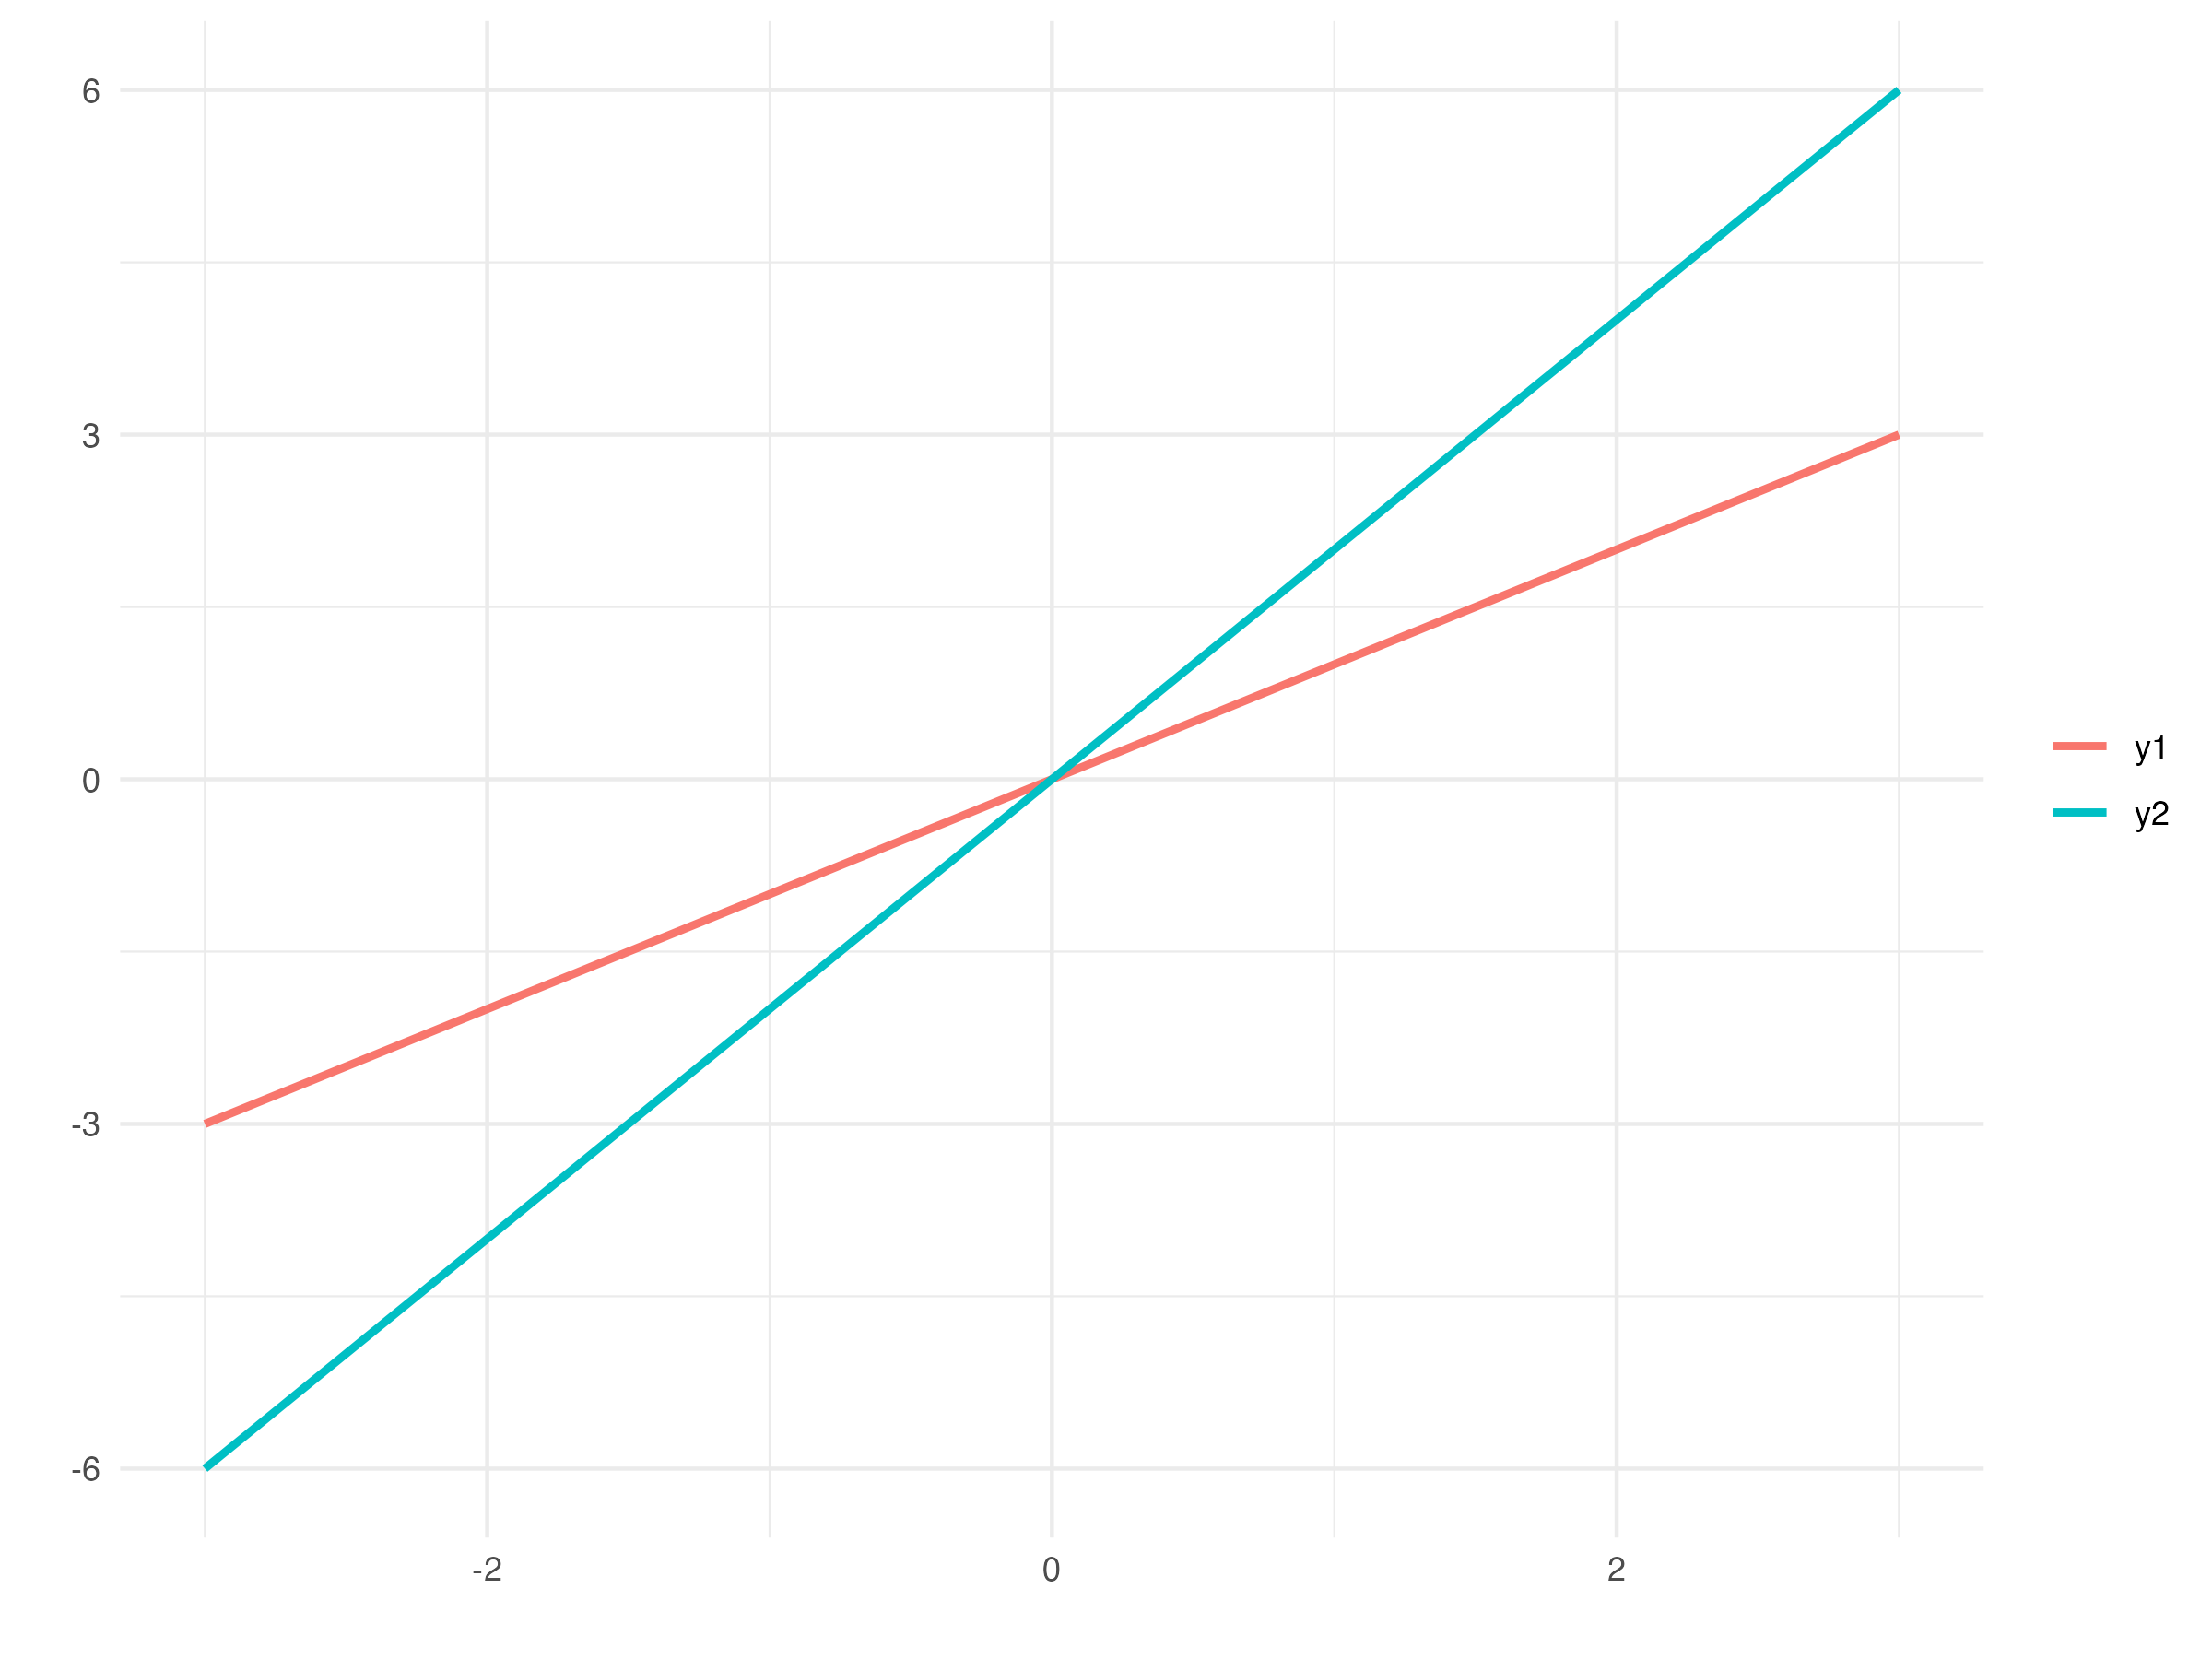
\includegraphics[width=\textwidth]{images/p_main_effect_ex1.png}
        \caption{Main terms as calculated via classical fANOVA for $g(x) = x_1 + 2 x_2 + x_1 x_2$.}
        \label{fig:main_effects_ex1}
    \end{minipage}%
    \hfill
    \begin{minipage}[t]{0.49\textwidth}
        \centering
        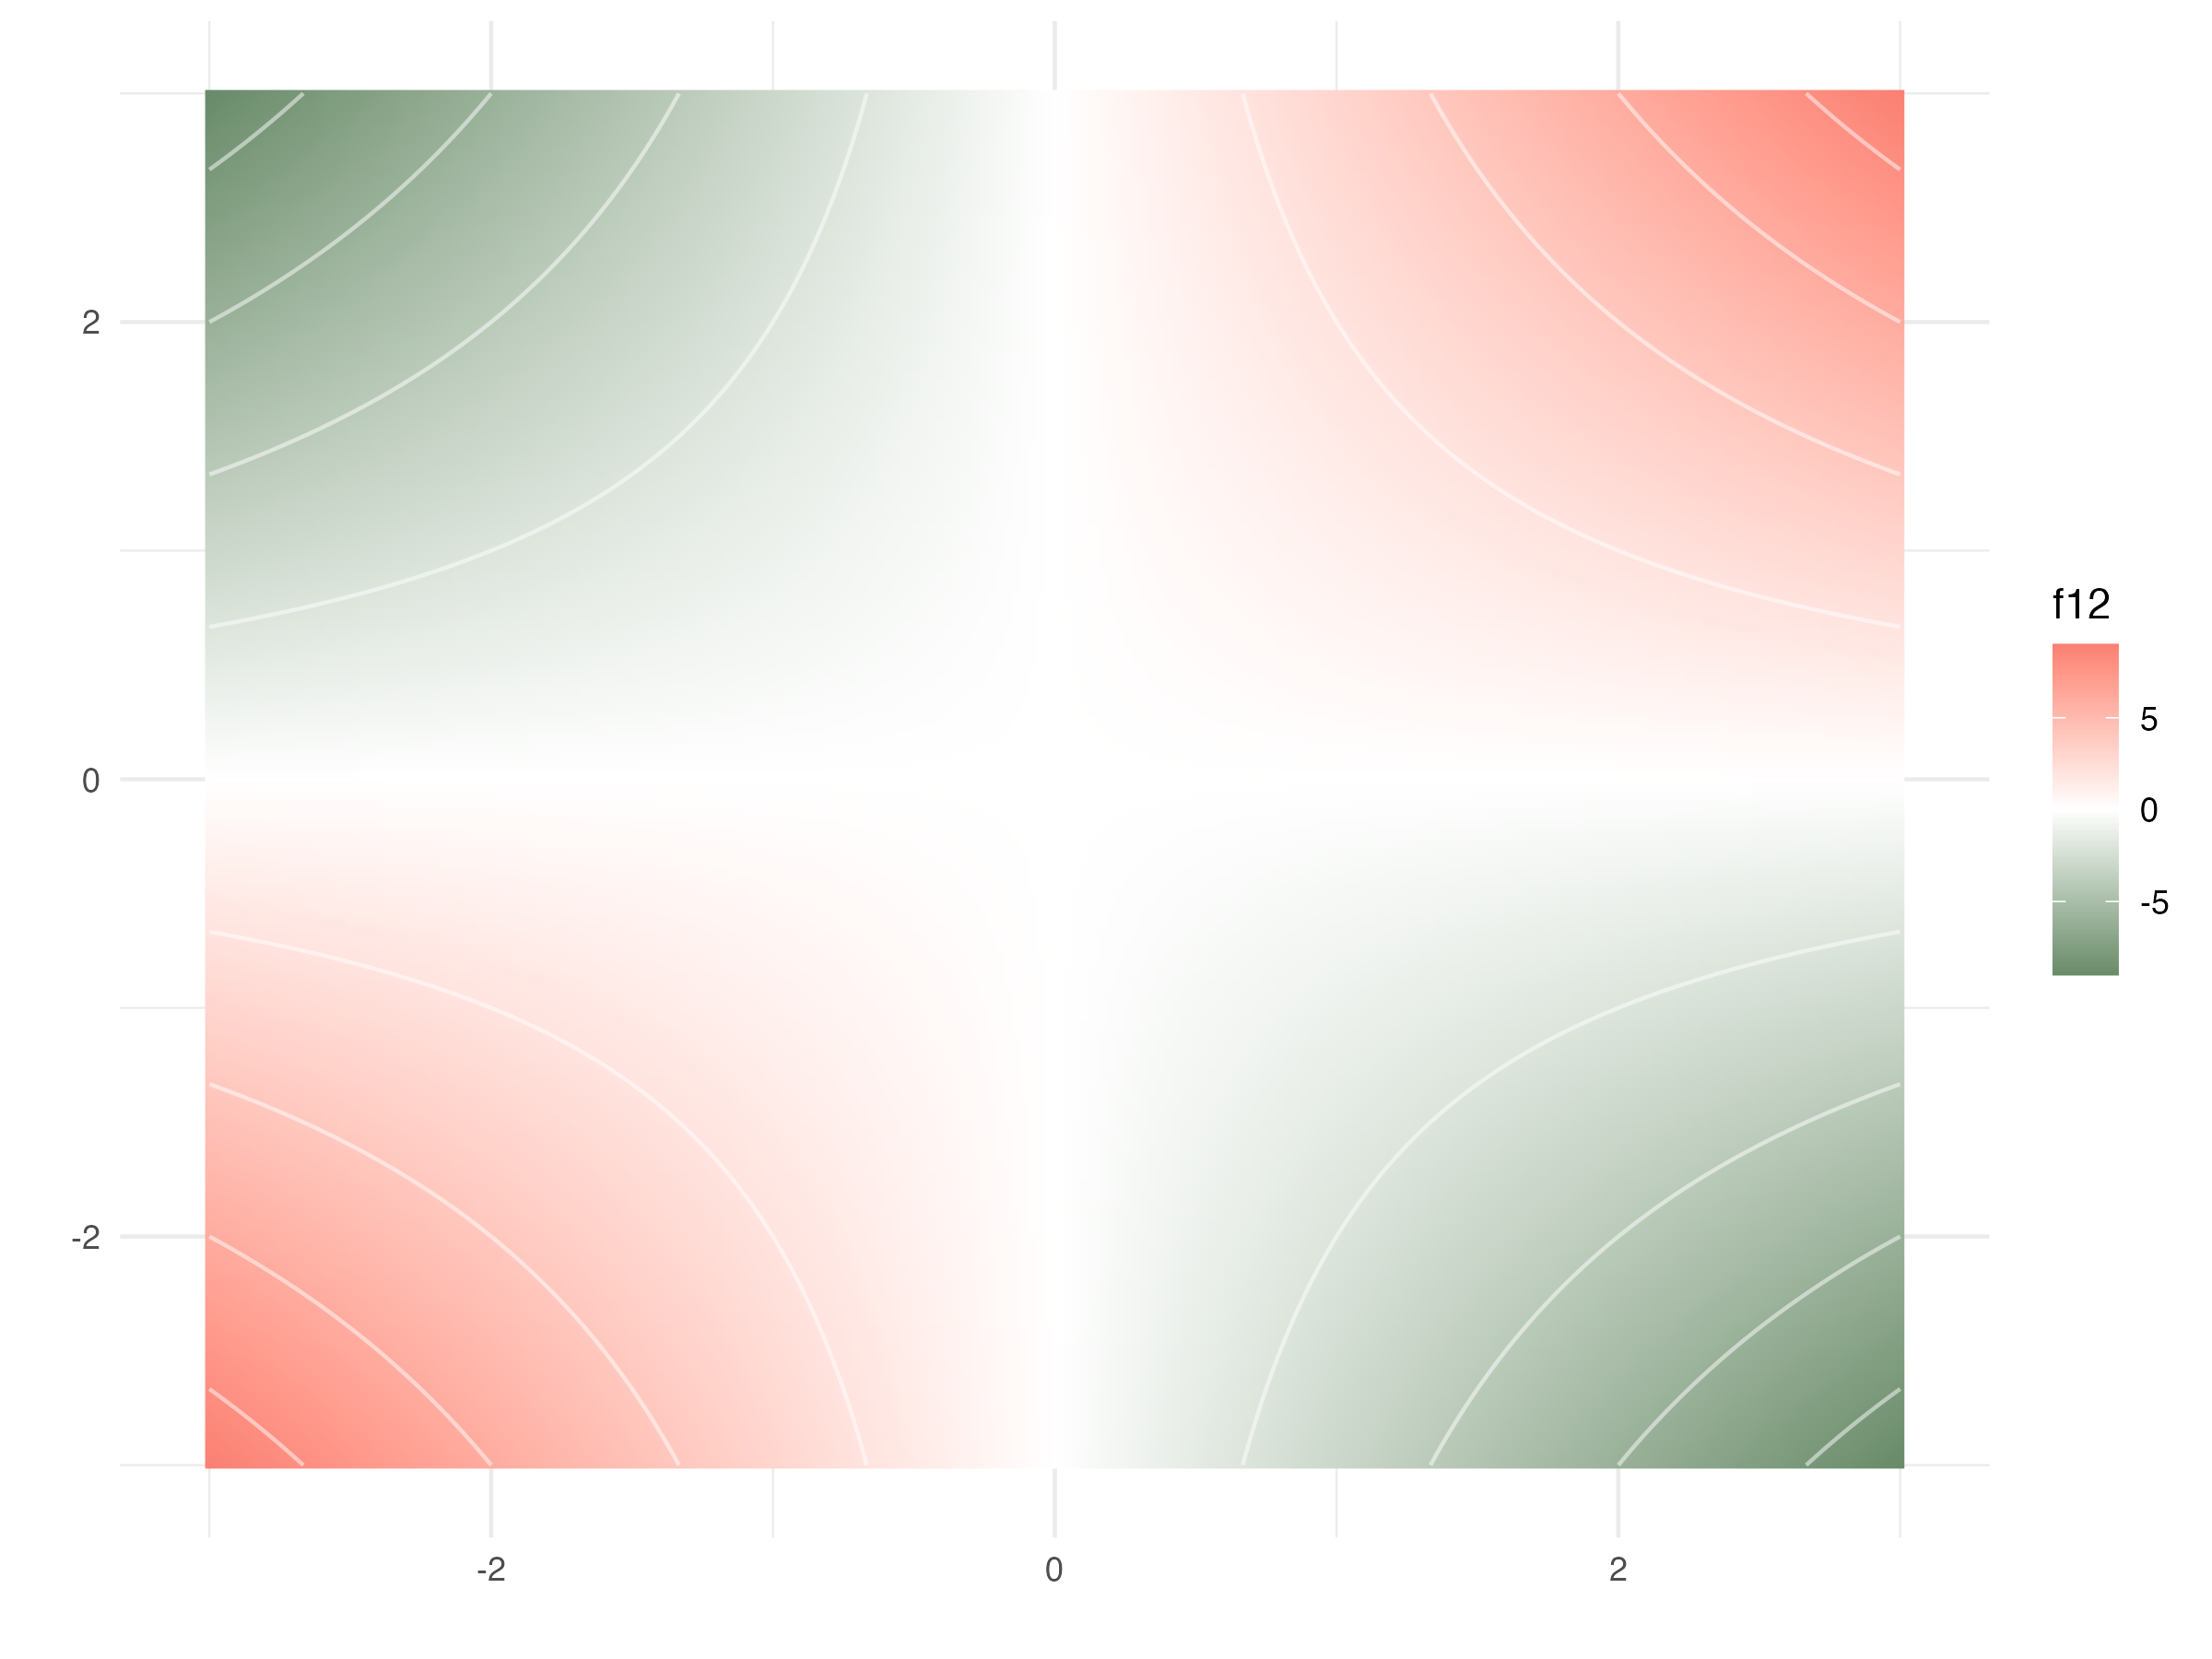
\includegraphics[width=\textwidth]{images/p_contour_ex1.png}
        \caption{Contour plot of $g(x) = x_1 + 2 x_2 + x_1 x_2$.}
        \label{fig:contour_ex1}
    \end{minipage}
\end{figure}

% \begin{figure}[htpb]
%     \centering
%     \begin{minipage}[t]{0.49\textwidth}
%         \centering
%         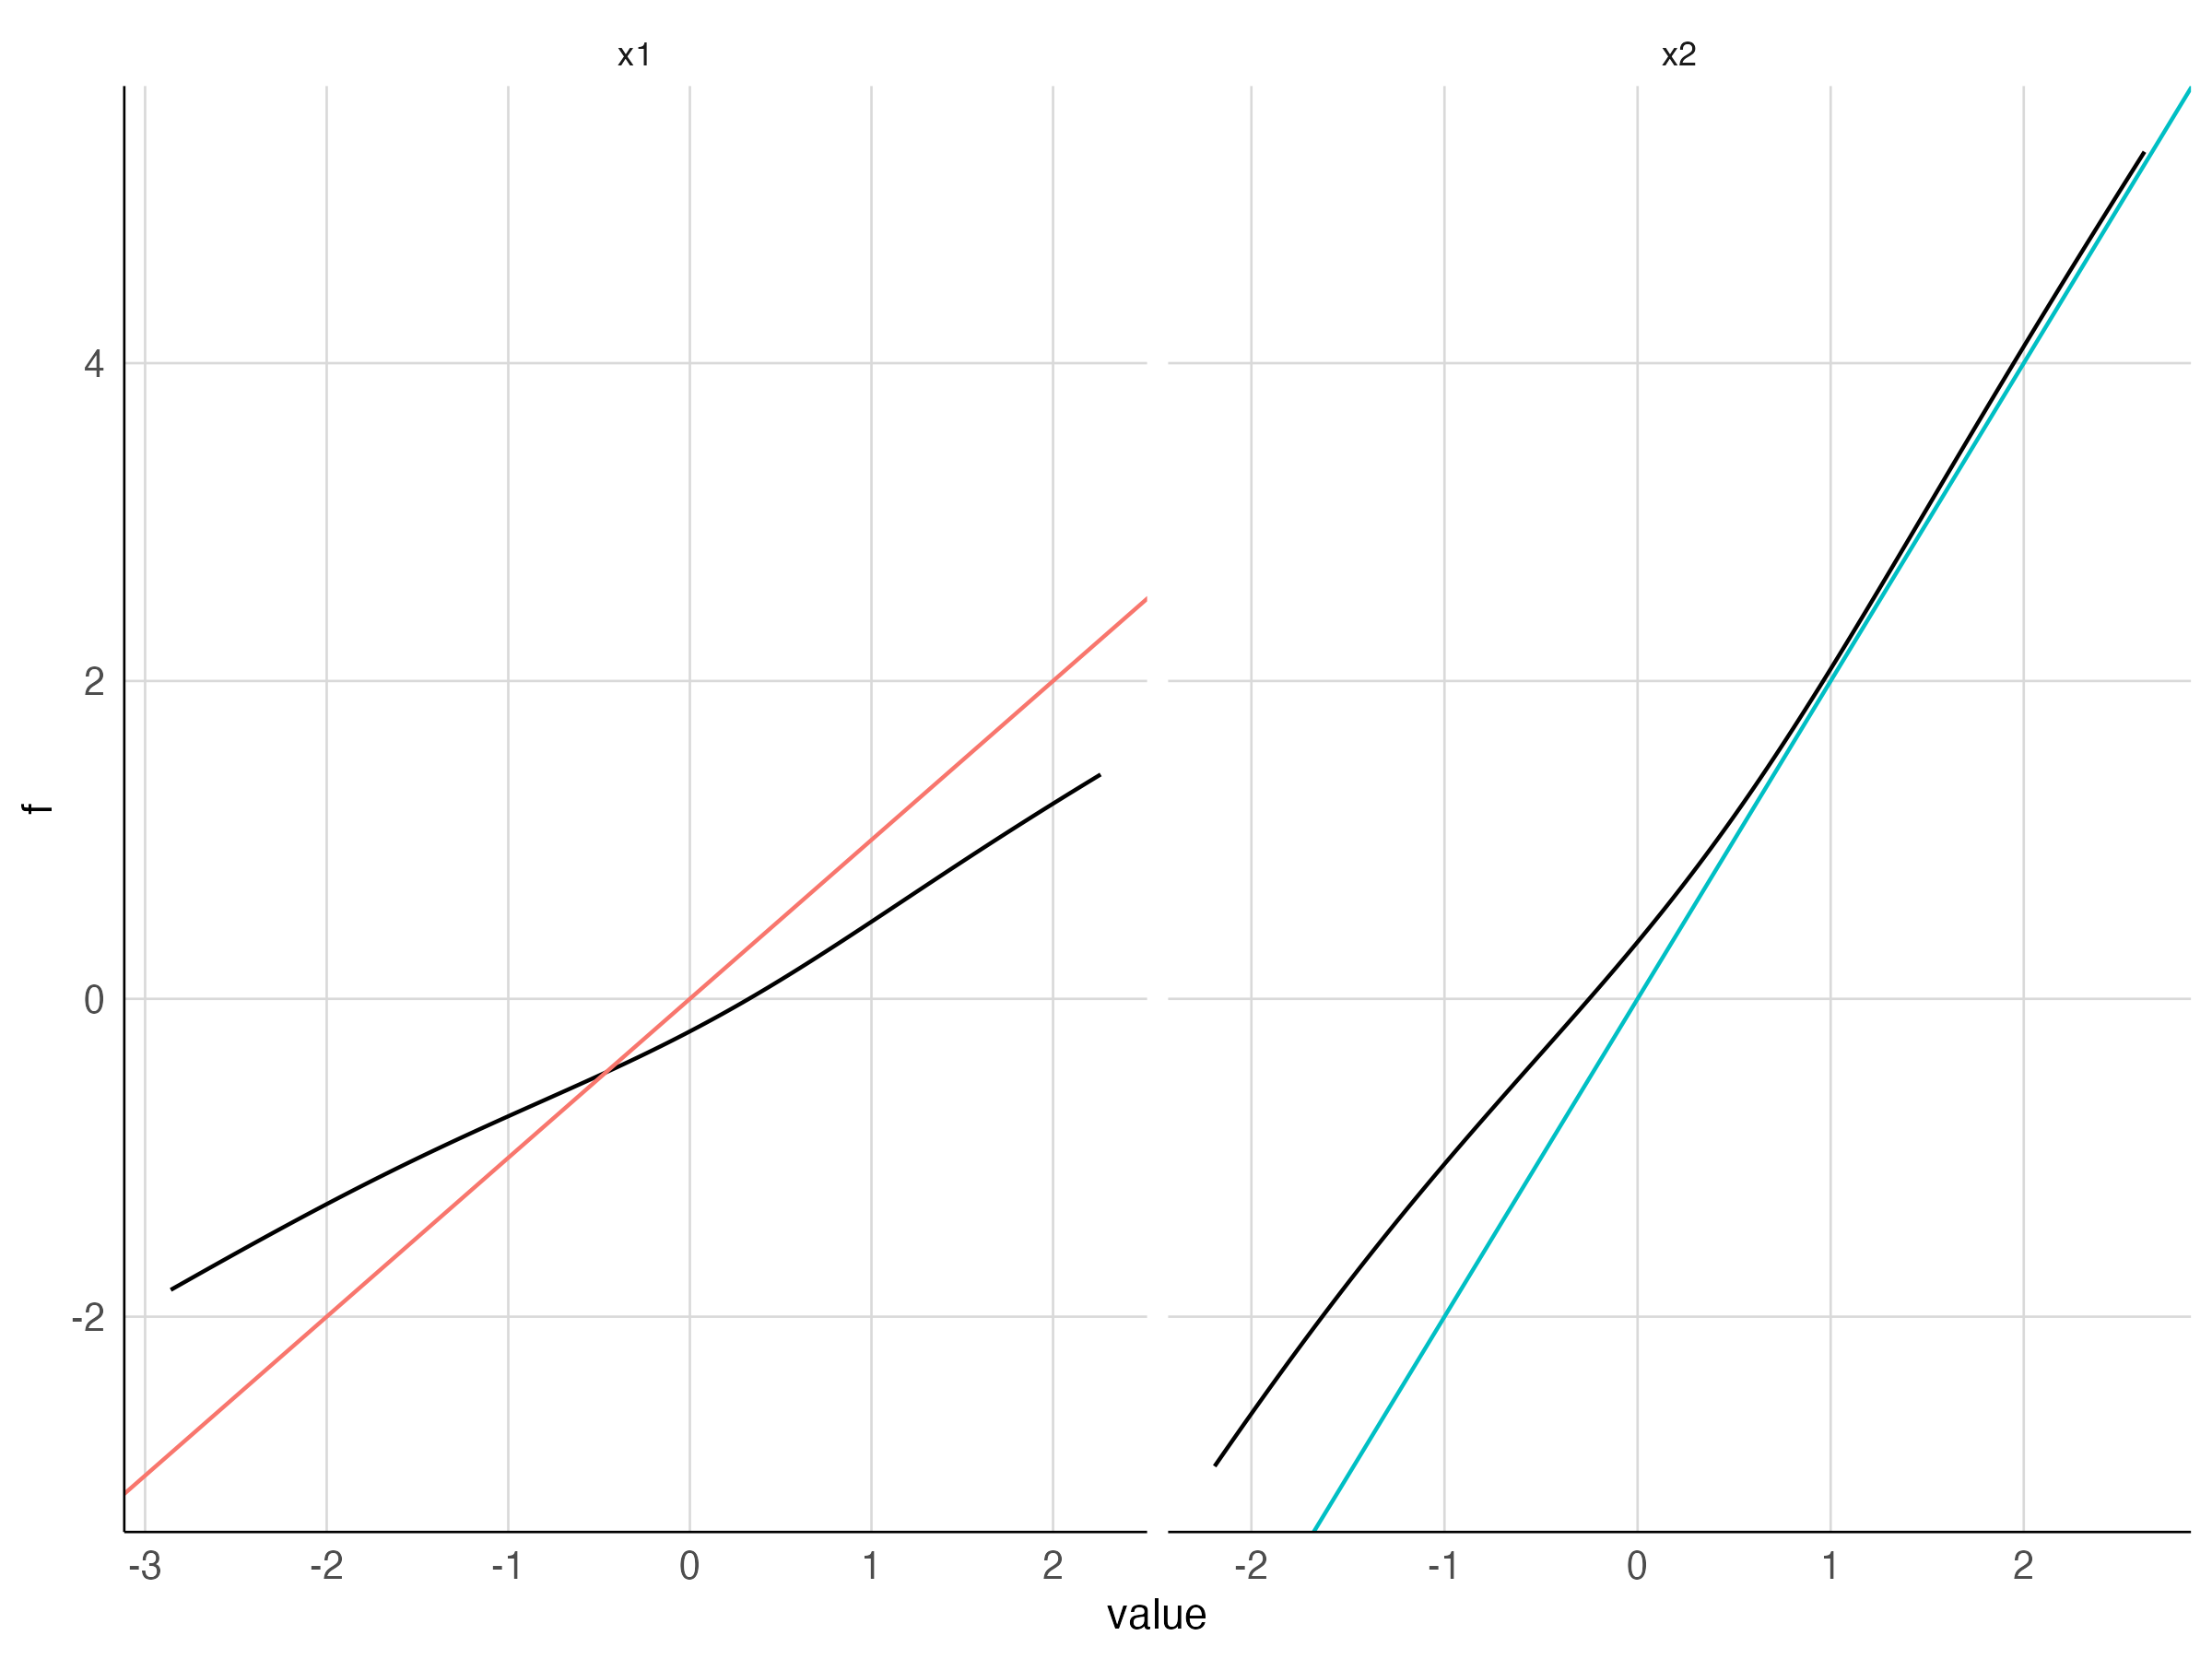
\includegraphics[width=\textwidth]{images/indep_150_main.png}
%         \caption{Estimation of Main terms as calculated via classical fANOVA for $g(x) = x_1 + 2 x_2 + x_1 x_2$ via Hooker method.}
%         \label{fig:indep_150_main}
%     \end{minipage}%
%     \hfill
%     \begin{minipage}[t]{0.49\textwidth}
%         \centering
%         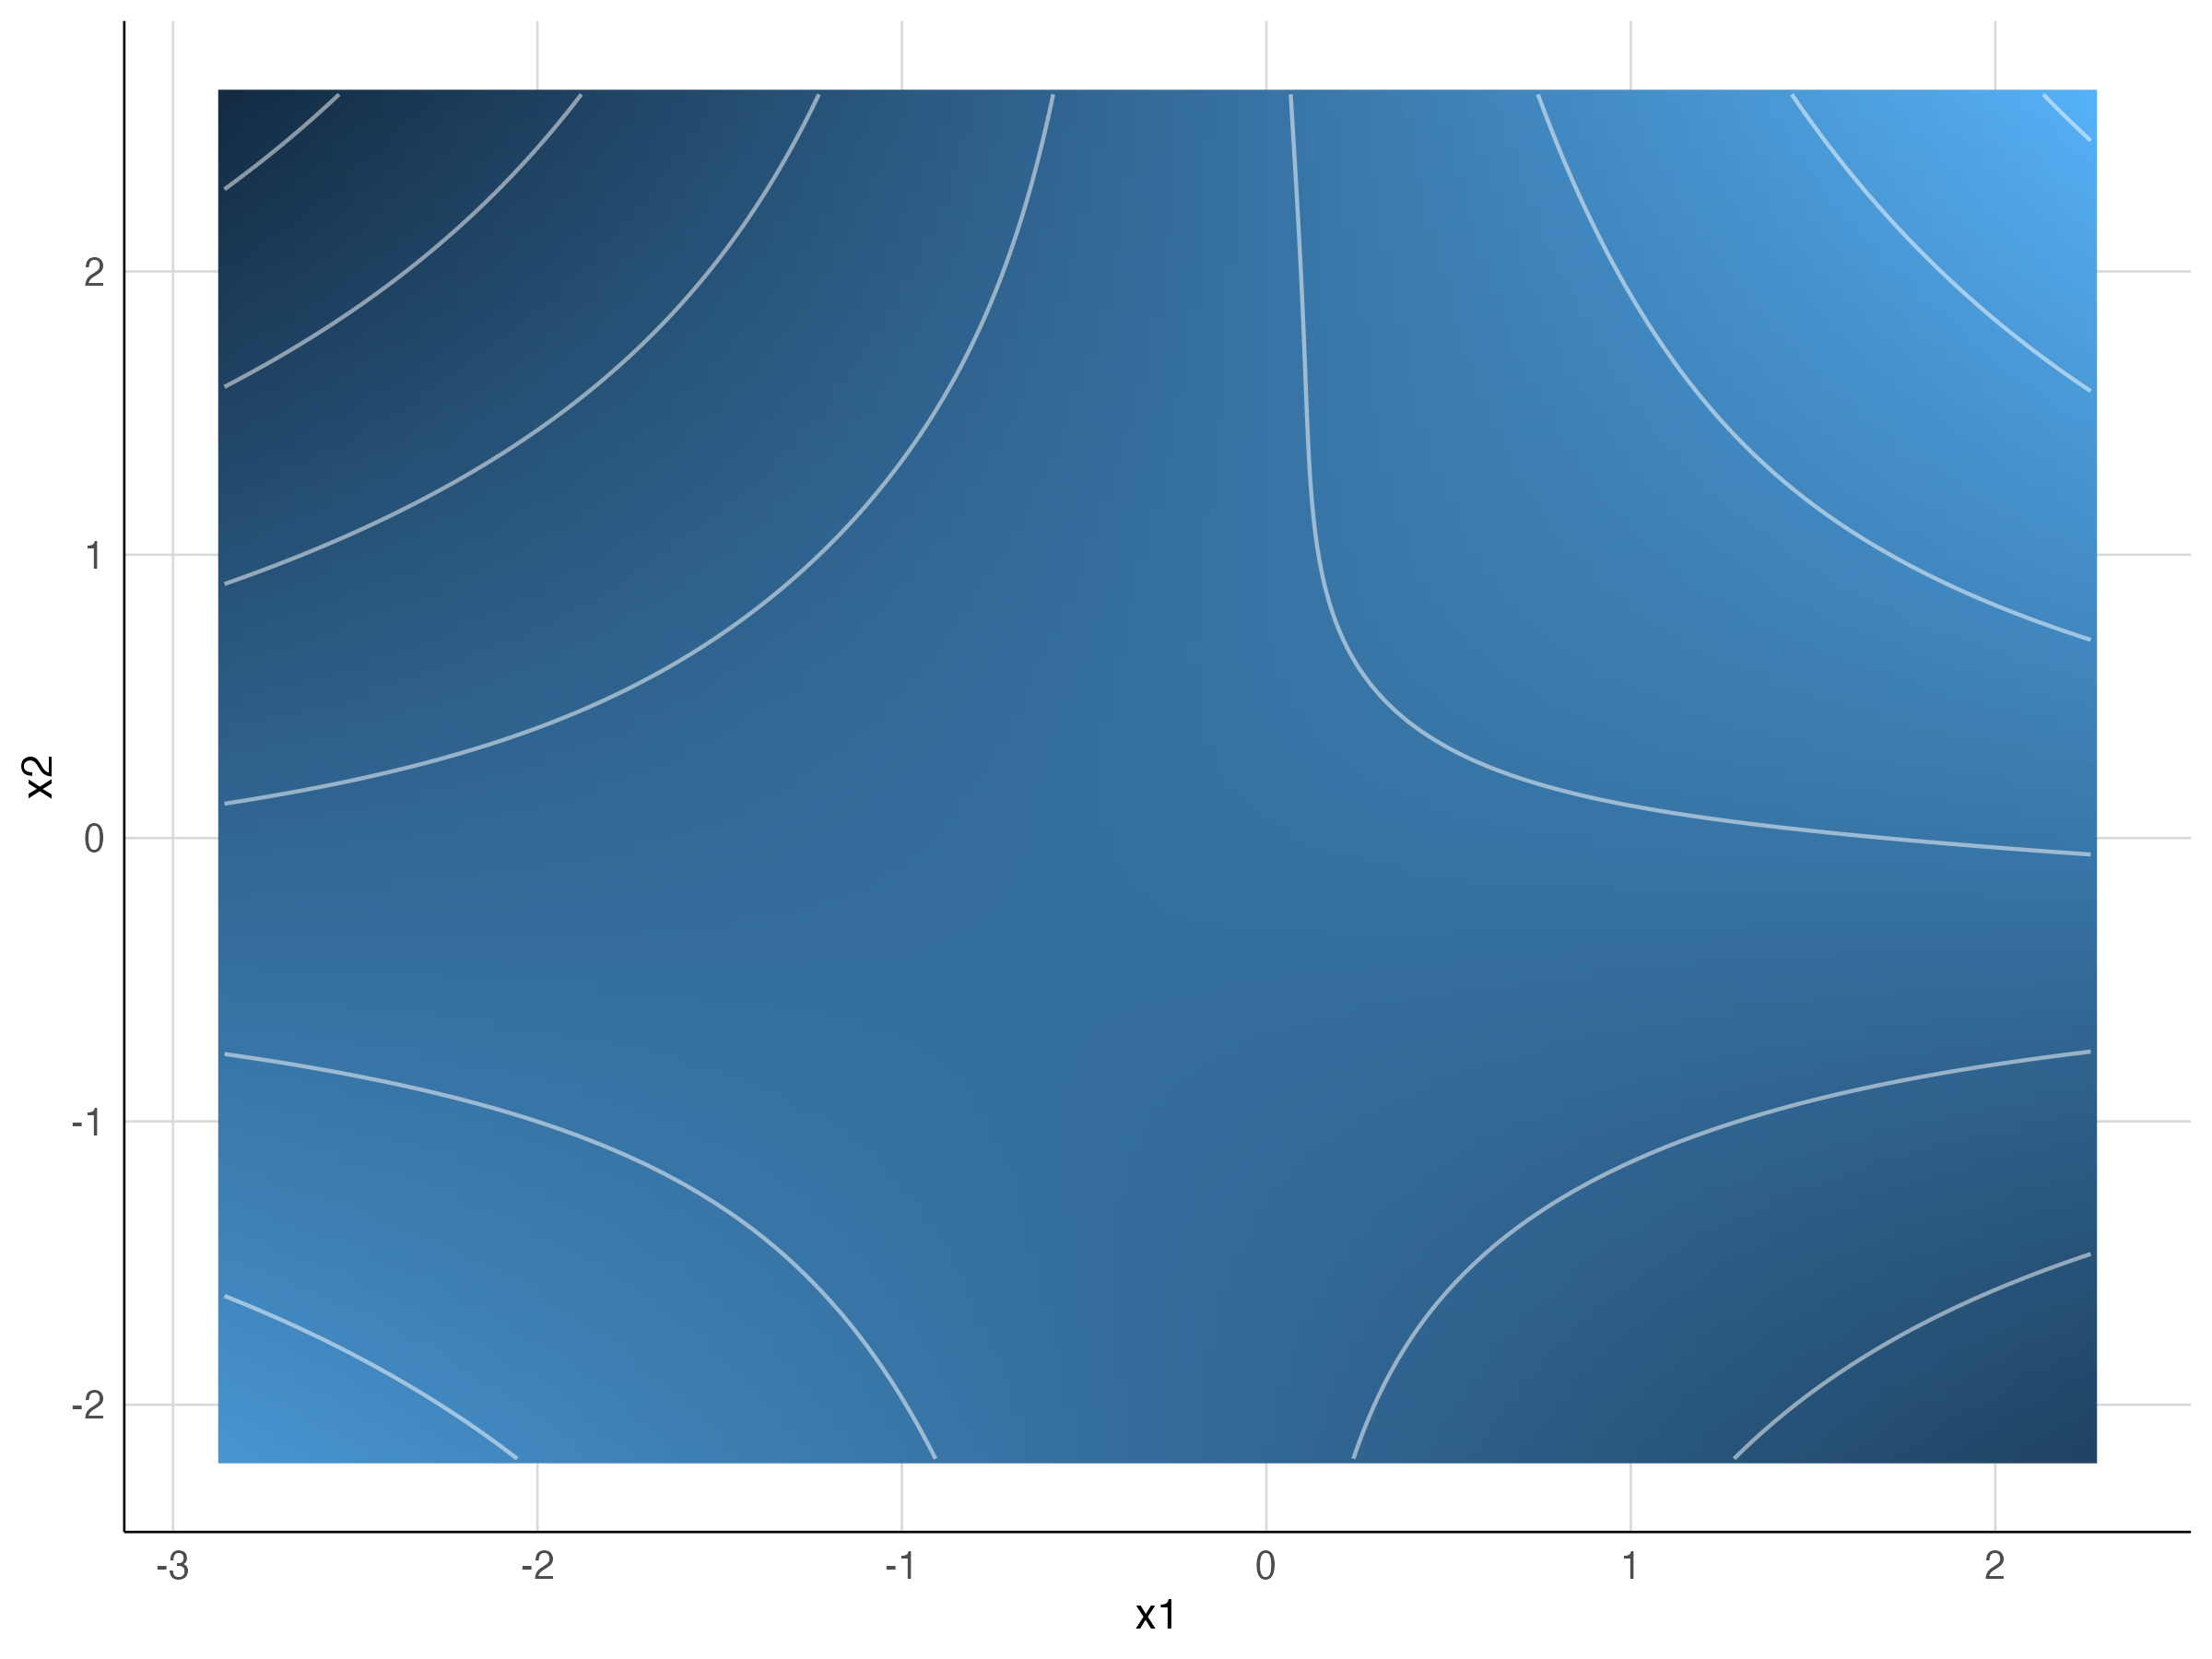
\includegraphics[width=\textwidth]{images/indep_150_interact.png}
%         \caption{Estimation of Contour plot of $g(x) = x_1 + 2 x_2 + x_1 x_2$ via Hooker method.}
%         \label{fig:indep_150_interact}
%     \end{minipage}
% \end{figure}

\subsubsection*{Standard MVN, linear function, interaction, dependent inputs}
% Zwei Plots für rho = 0.6 nebeneinander, jeweils halbe Breite
\begin{figure}[htpb]
    \centering
    \begin{minipage}[t]{0.49\textwidth}
        \centering
        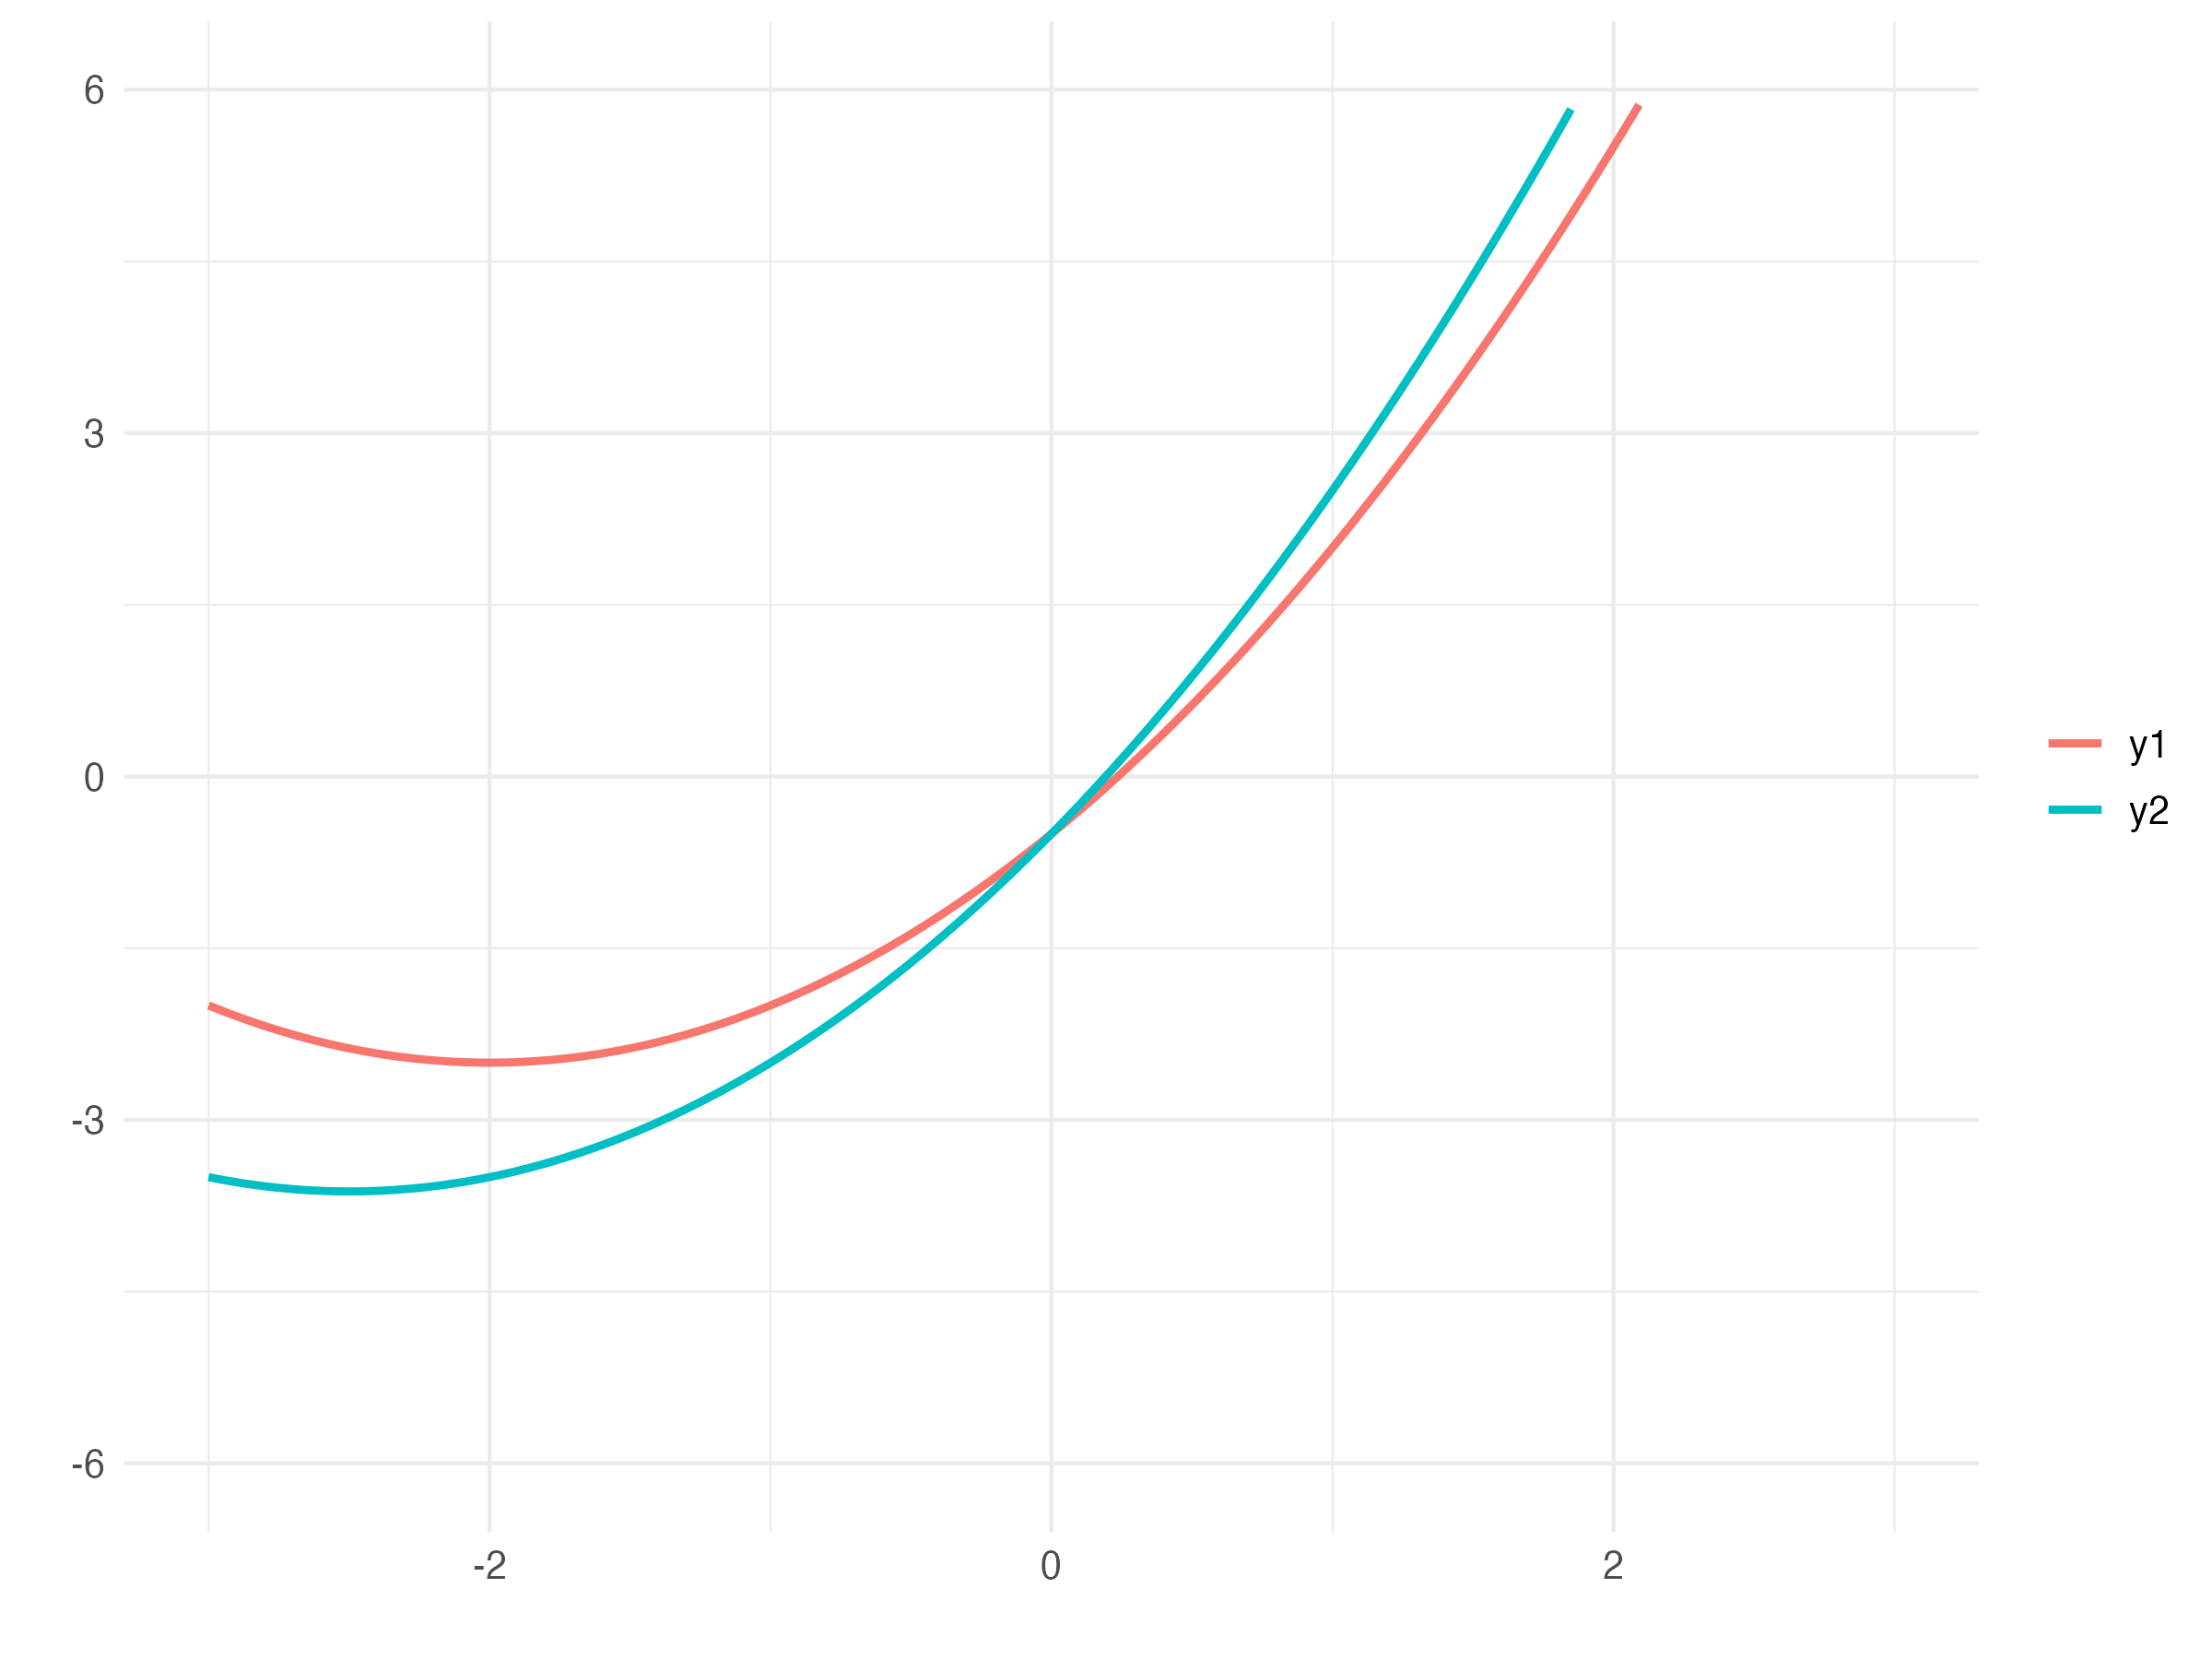
\includegraphics[width=\textwidth]{images/hoeffding_rho05.png}
        \caption{Hoeffding decomposition of $g(x) = x_1 + 2 x_2 + x_1 x_2$ with $\rho = 0.5$.}
        \label{fig:hoeffding_rho05}
    \end{minipage}%
    \hfill
    \begin{minipage}[t]{0.49\textwidth}
        \centering
        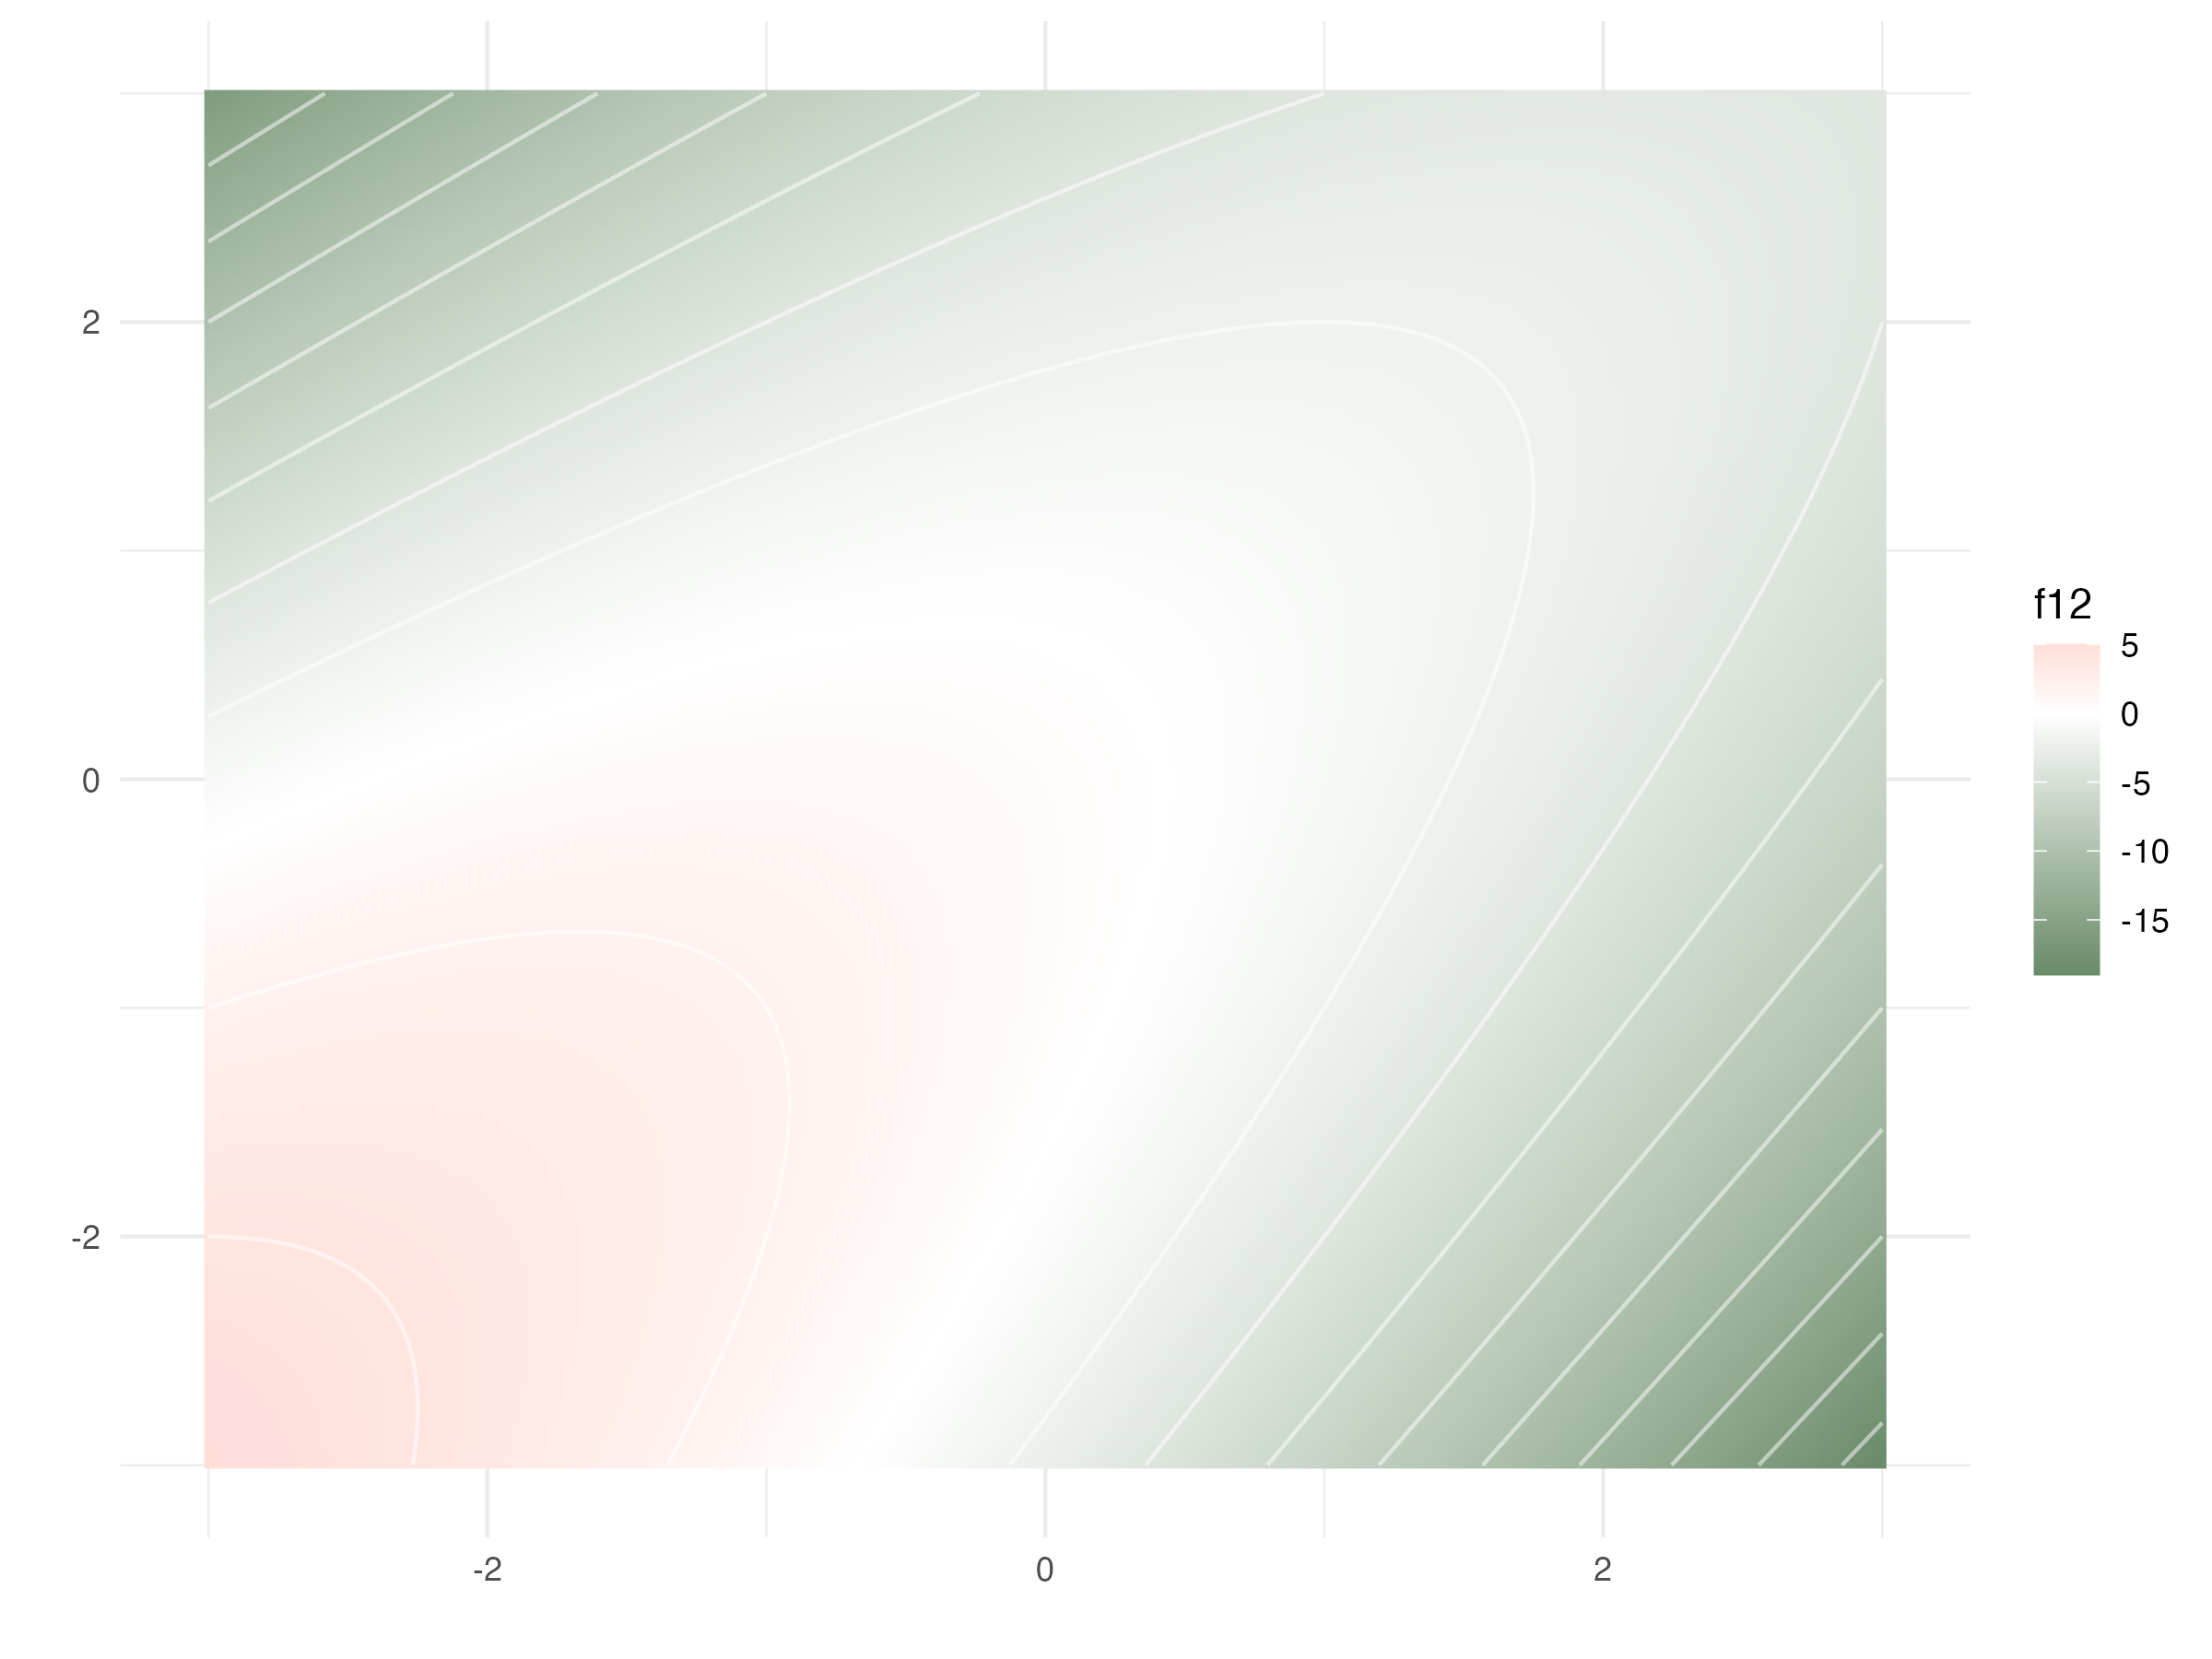
\includegraphics[width=\textwidth]{images/hoeffding_contour_rho05.png}
        \caption{Contour plot of $g(x) = x_1 + 2 x_2 + x_1 x_2$ with $\rho = 0.5$.}
        \label{fig:hoeffding_contour_rho05}
    \end{minipage}
\end{figure}

\subsubsection*{Estimated generalized fANOVA components}
\begin{figure}[htpb]
    % insert g1_1 and g1_2 as minipages
    \centering
    \begin{minipage}[t]{0.49\textwidth}
        \centering
        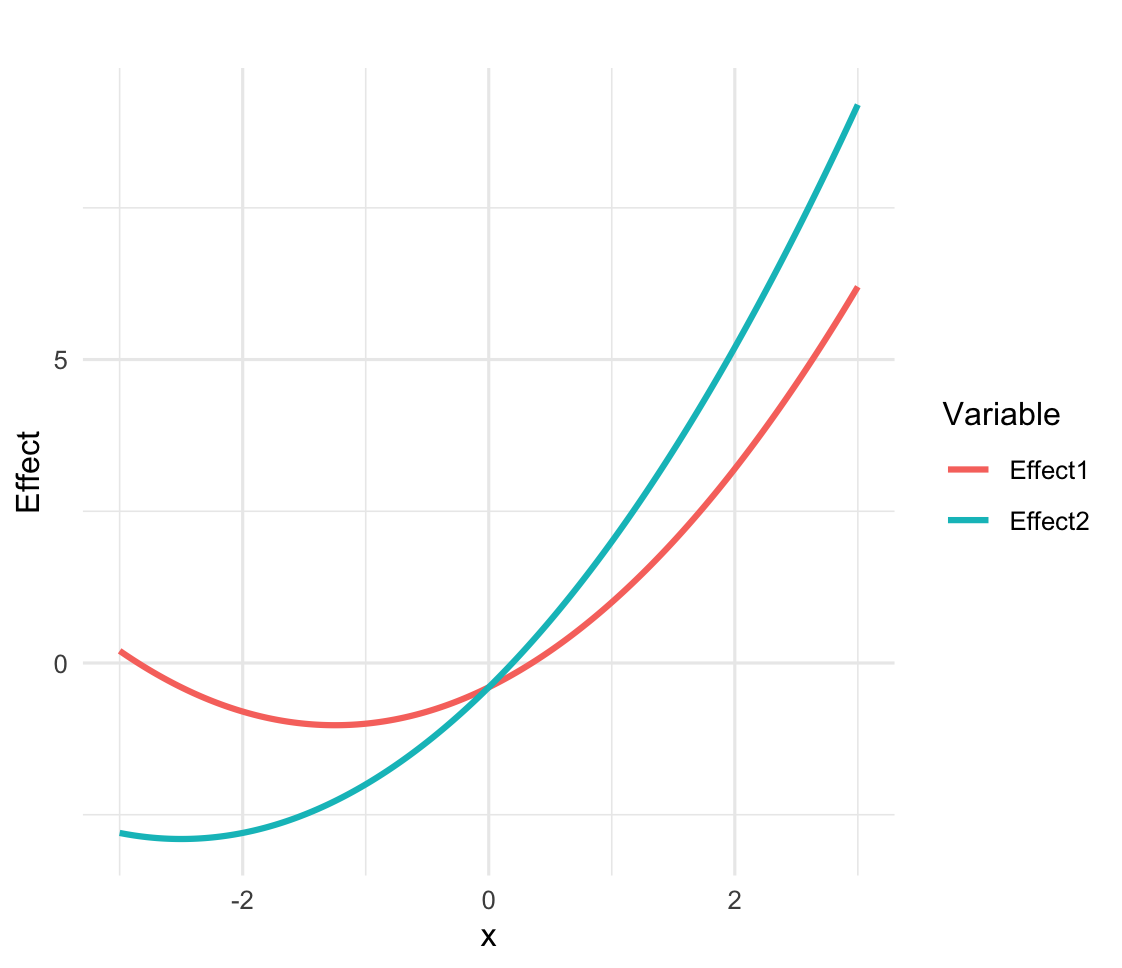
\includegraphics[width=\textwidth]{images/gpt_func_main.png}
        \caption{Generalized main effects for $g(x) = x_1 + 2 x_2 + x_1 x_2$ with dependent inputs, $\rho = 0.5$.}
        \label{fig:dep_150_main}
    \end{minipage}%
    \hfill
    \begin{minipage}[t]{0.49\textwidth}
        \centering
        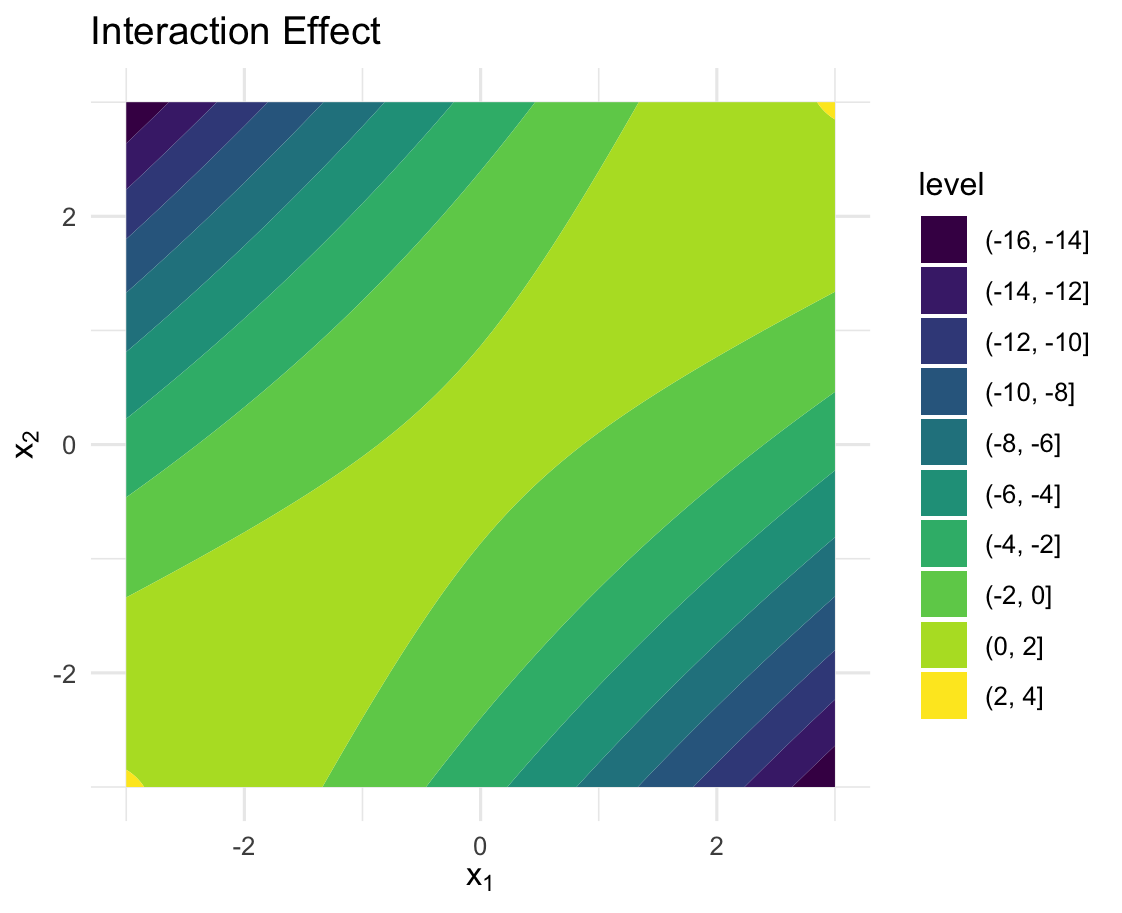
\includegraphics[width=\textwidth]{images/gpt_func_interaction.png}
        \caption{Contour plot of generalized interaction term for $g(x) = x_1 + 2 x_2 + x_1 x_2$ with dependent inputs, $\rho = 0.5$.}
        \label{fig:dep_150_interact}
    \end{minipage}
\end{figure}


\subsubsection*{Standard MVN, linear function, interaction, non-centred inputs}
Next, instead of a standard MVN distribution assumption for the inputs, we allow for non-centred inputs. This is to confirm that the fANOVA decomposition manages to yield zero mean components, even when inputs are not centred.
\(g = a + X_1 + 2X_2 + X_1 X_2\)
\[
\begin{pmatrix}
X_1 \\
X_2
\end{pmatrix}
\sim \mathcal{N}\left(
\begin{pmatrix} \mu_1 \\ \mu_2 \end{pmatrix},
\begin{pmatrix}
1 & 0 \\
0 & 1
\end{pmatrix}
\right).
\]
From the properties of the MVN, we know that marginal distributions are standard normal:
\[
X_i \sim \mathcal{N}(0, 1) \quad \text{for } i = 1, 2
\]

We also know that the conditional distributions are given by:
\[
X_1 \mid X_2 = x_2 \sim \mathcal{N}(\mu_1, 1), \quad
X_2 \mid X_1 = x_1 \sim \mathcal{N}(\mu_2, 1)
\]

We can now compute the classical fANOVA components as follows:
\begin{align*}
    y_{\emptyset} &= \mathbb{E}[g(X)] = a + \mu_1 + 2\mu_2 + \mu_1 \mu_2, \\
    y_1 &= \mathbb{E}[g(X) \mid X_2 = x_2] - y_{\emptyset}= a + 2\mu_2 + x_1 + x_1 \mu_2 - y_{\emptyset} \\
    &= x_1 ( 1 + \mu_2) - \mu_1 \mu_2 - \mu_1, \\
    y_2 &= \mathbb{E}[g(X) \mid X_1 = x_1] - y_{\emptyset} = a + \mu_1 + 2x_2 + x_2 \mu_1 - y_{\emptyset} \\
    &= x_2 (2 + \mu_1) - \mu_1 \mu_2 - 2 \mu_2, \\
    y_{12} &= g(x_1, x_2) - y_{\emptyset} = x_1x_2 - \mu_2 x_1 - \mu_1 x_2 + \mu_1 \mu_2.      
\end{align*}
We recognize that each fANOVA components is shifted by constants (that are formed from the conditional and unconditional expected values of the input variables). 

It is easy to verify that non-constant terms have mean zero:
\begin{align*}
    \mathbb{E}[y_1] &= \mathbb{E}[X_1 (1 + \mu_2) - \mu_1 \mu_2 - \mu_1] = (1 + \mu_2) \mathbb{E}[X_1] - \mu_1 \mu_2 - \mu_1 = 0, \\
    \mathbb{E}[y_2] &= \mathbb{E}[X_2 (2 + \mu_1) - \mu_1 \mu_2 - 2\mu_2] = (2 + \mu_1) \mathbb{E}[X_2] - \mu_1 \mu_2 - 2\mu_2 = 0, \\
    \mathbb{E}[y_{12}] &= \mathbb{E}[X_1X_2] - \mu_2 \mathbb{E}[X_1] - \mu_1 \mathbb{E}[X_2] + \mu_1 \mu_2 = 0.
\end{align*}
Varying the mean of MVN inputs will result in shifted fANOVA components. Varying the variance of intput variables will not change the fANOVA decomposition and is therefore not investigated further.
% Input: Poisson/ Exponential/ Beta/ etc. not centred, independent

\paragraph{Non-additive functions}
These functions demonstrate that fANOVA does not assume additive structure and can identify purely interactive effects. If variables only appear in interaction terms, their main effects vanish:
\[
f_2(x) = x_1 \cdot x_2 \cdot x_3 \cdot x_4
\]


\subsubsection*{Uniform, quadratic, no interaction}
Let us also try out another function $g(x_1, x_2) = a + x_1 + x_2^2$; to see how fANOVA deals with quadratic main effects. 
We will also change the distribution of the inputs. Lets us consider two independent random variables with uniform distribution over the interval \([-1, 1]\), meaning they are already centred. We calculate:
\begin{align*}
y_\emptyset &= \mathbb{E}[g(X_1, X_2)] = a + \mathbb{E}[X_1] + \mathbb{E}[X_2^2] = a + 0 + \tfrac{1}{3} = a + \tfrac{1}{3} \\
y_1(x_1) &= \mathbb{E}[g(x_1, X_2)] - y_\emptyset = a + x_1 + \tfrac{1}{3} - \left(a + \tfrac{1}{3}\right) = x_1 \\
y_2(x_2) &= \mathbb{E}[g(X_1, x_2)] - y_\emptyset = a + 0 + x_2^2 - \left(a + \tfrac{1}{3}\right) = x_2^2 - \tfrac{1}{3} \\
y_{1,2}(x_1, x_2) &= g(x_1, x_2) - y_\emptyset - y_1(x_1) - y_2(x_2) = a + x_1 + x_2^2 - \left(a + \tfrac{1}{3} + x_1 + x_2^2 - \tfrac{1}{3}\right) = 0
\end{align*}

\newpage

\section{Conclusion}\label{sec:conclusion}
% Recaps of what I did
% 1. gave historical context of fANOVA by showing origins of the method and how it evolved over time
% We started by working through the historical context of the fANOVA decomposition. We explored the origins of the fANOVA method rooted in mathematical work by \cite{hoeffding1948} and \cite{sobol1993sensitivity}. We saw how the method was picked up by following researchers in different contexts.

% 2. formal introduction, to classical fANOVA
% synthesise multiple sources into one clean, general but not 
% too general formulation of the method
% looked at key properties that characterize fANOVA + distinguish it from other IML methods

% --->> could work out a bit more (for now mostly conceptually)
% uniqueness of fANOVA in comparison to other methods
% e.g. say that it is a global technique, decomposes the function
% it is model agnostic, global etc.

% 3. generalization of fANOVA
% we saw how classical fANOVA breaks down under dependent inputs
% weak independence might not be problem but if features are strongly correlated fANOVA will yield misleading results
% the generalization is in the end doing nothing other than letting go of the product type probability measure 
% but constructing components that still satisfy the nice properties and add up to the original function is not trivial 
% there are multiple ways to generalize the components, we mostly
% focused on work by Hooker and Rahman


% we unified different formulations of the method using the parallel
% between conditional expected value and orthogonal projections
% this is the key to bringing different formulations together and also generlizing the idea of fANOVA
% to different scenarios

% approximation of fANOVA done via sampling, lagrange multiplier etc.

The fANOVA decomposition is a foundation method that has been studied from many perspectives, with recent interest driven by its potential in model interpretability. Its key strength lies in producing terms that represent the unique contribution of each variable or interaction, cleanly separated from one another without mixing effects.\par

Despite being established in the literature, we found a lack of unified formalization and notational clarity in the literature, which we aimed to address in this work.\par

We began by revisiting the classical fANOVA decomposition, bridging Sobols initial formulation with more recent developments. We filled small gaps in mathematical proofs and established a direct connection to conditional expectations and orthogonal projections, which we argue is key to unifying different existing notations and formal approaches. Alongside the functional decomposition, we presented the variance decomposition, which underpins Sobol indices and links the fANOVA structure to sensitivity analysis.\par

Next, we extended the decomposition to dependent input variables. Here, multiple approaches exist; we focused on the frameworks of \cite{hooker2007} and \cite{rahman2014}. Using an illustrative example, we encountered the close relation between the fANOVA and Hoeffding decompositions and demonstrated that obtaining interpretable fANOVA components under dependence requires careful constraint selection. We also noted that closed-form solutions for the generalized components are difficult to obtain in practice and remain an open problem. Nevertheless, the associated variance decomposition still holds, allowing for the construction of generalized Sobol indices.\par

To complement the theoretical work, we visualized fANOVA components for simple polynomial functions with Gaussian inputs. These visualizations illustrated how fANOVA separates effects, but were limited to simple functions and Gaussian inputs.\par

This work did not present a full numerical treatment of Sobol indices, only touching on variance decomposition as their foundation. Our empirical demonstrations were restricted to toy problems; applying fANOVA in practice will require estimation methods suitable for trained models on real data. We also briefly mentioned the ability of fANOVA to purify interaction effects \citep{lengerich2020} and its relation to other interpretability techniques (e.g., PD, Shapley values \citep{fumagalli2025}) but did not explore these connections in depth.\par

Future work could extend Rahman’s polynomial expansion approach to more complex polynomials and non-Gaussian input distributions, and further investigate mathematical connections to other interpretability frameworks.
Additionally, a lack of publicly available software for performing fANOVA remains a barrier to its widespread adoption, so developing robust, open-source implementations would be an important step toward enabling its use in practical model interpretability.

% Recap: fANOVA is a foundation method studied from many perspectives; most recently researchers caught interest in fANOVA for its potential in model interpretability - what makes it special is that the fANOVA terms represent the unique contribution of each variable or interaction - they are cleanly separated from each other and do not mix up.
% Though so widely used we found a lack of unified formalization and notational clarity, which we hope to have provided with this work.\par
% We started with the classical fANOVA decomposition; well-known in literature \cite{rahman2014} but we filled some small gaps in mathematical proofs, and wrote out the paralel to conditional expected value and orthogonal projections, which is the key to unifying different notations and approaches to the formalization of fANOVA.
% We briefly adressed the variance decomposition, which goes hand in hand with the functional decomposition and is the foundation of Sobol indices.\par
% We then generalized the fANOVA decomposition to dependent inputs. Here different approaches exist, and we focused on the work by \cite{hooker2007} and \cite{rahman2014}. Based on an example we saw that the fANOVA decomposition is closely related to Hoeffding decomposition and to obtain the real fANOVA components under independence with their clear interpretation it is necessary to construct a careful set of constraints.
% Obtaining a closed form solution for the generalized components is challenging in most cases and remains an open problem. Though more complex the variance decomposition still works in principle and allows for the construction of generalized Sobol indices.\par
% Lastly, we experimented with visualizing the fANOVA components of different functions, while we stayed within the realm of two degree polynomials with Gaussian inputs.\par
% % Limitations of this work:
% % did not really present Sobol indices, only mentioned the variance decomposition
% % Illustrated fANOVA with toy example in really limited setting; would be intersting to train a model on real data and really apply fANOVA decomposition; for this however we need an estimation approach
% % In the final section it was elluded briefly: fANOVA and how it can purify interactions, did not go into depth but this is an interesting topic highly relevant to fANOVA and interpretability
% % Briefly contrasted fANOVA to other IML methods here and there but did not formally compare to other methods; would be very interesting to examine this from a mathematical pespective: direct connection to partial dependence and recent work also shows mathematical connection to Shapley values \cite{fumagalli2025}.
% For future work it would be interesting to study the extension of Rahman's polynomial expansion approach for other distribution assumptions and more complex polynomials. Moreover, as we argued in the end, there is a lack of software implementations for fANOVA decomposition, which is a barrier to its application in model interpretability.


% fANOVA powerful theory, sound mathematical foundation, but without standardized software implementation application to IML difficult.
% Parallels to Shapley values, unified under a game theoretic approach; \cite{fumagalli2025} recently established this parallel, would be very interesting to investigate further.
% Use Rahmans methods and extend it to different distribution assumptions.



% ------------------------------------------------------------------------------
% BIBLIOGRAPHY -----------------------------------------------------------------
% ------------------------------------------------------------------------------
\addcontentsline{toc}{section}{References}
\RaggedRight
\bibliographystyle{dcu}
\bibliography{bibliography_2,bibliography_manual}
\newpage


% ------------------------------------------------------------------------------
% APPENDIX ---------------------------------------------------------------------
% ------------------------------------------------------------------------------
    
\pagenumbering{Roman}

\setcounter{page}{5} % CHANGE

\appendix

\section{Appendix}
\label{app}
\section*{Square Integrability of \( f_1(x_1) \)}

For now we want to show that the single fANOVA term \( f_1(x_1) \) is square integrable, given that the original function $f(x) \in \mathcal{L}^2$. We need to show that:
\[
\int |f_1(x_1)|^2 \, dx_1 < \infty
\]

The single fANOVA term is defined as:
\[
f_1(x_1) = \int f(x) \, dx_{-1} - f_0
\]

We take the squared norm, and integrate w.r.t. \( x_1 \) to use the Cauchy-Schwarz inequality:
\[
\int |f_1(x_1)|^2 \, dx_1 
= \int \left| \int f(x) \, dx_{-1} - f_0 \right|^2 dx_1
\]

\[
= \int | (\int f(x) \, dx_{-1})^2 
- 2 \int f(x) \, dx_{-1} f_0 
+ f_0^2 | dx_1
\]

Break this into three terms:
\begin{align*}
(1): &\quad \int \left| \int f(x) \, dx_{-1} \right|^2 dx_1 
\leq \int \left( \int 1^2 \, dx_{-1} \right) \left( \int |f(x)|^2 \, dx_{-1} \right) dx_1 
= \int |f(x)|^2 \, dx < \infty \\
\\
(2): &\quad 2 \int \left( \int f(x) \, dx_{-1} \right) f_0 \, dx_1 
= 2 f_0 \int \left( \int f(x) \, dx_{-1} \right) dx_1 
= 2 f_0^2 < \infty \\
\\
(3): &\quad \int f_0^2 \, dx_1 = f_0^2 < \infty
\end{align*}

Since each term (1)–(3) is finite, and \( \int |f_1(x_1)|^2 dx_1 \) is a linear combination of them: \(\int |f_1(x_1)|^2 dx_1 < \infty\)



% We want to show that the square integrability of the original function \( f \) implies the square integrability of the fANOVA terms \( f_0, f_1, \ldots, f_k \).
% For simplicity, we restrict ourselves to a fixed number of dimensions and therefore a fixed set of indices $i = 1, 2, 3, 4$.
% To start, we define the cumulative fANOVA decomposition as follows:
% \begin{align}
%     g_1(x) &= \int f(x) dx_{-1} = \int f(x) dx_2 dx_3 dx_4 \\
%     g_2(x) &= \int f(x) dx_{-2} = \int f(x) dx_1 dx_3 dx_4 \\
%     g_{1,2}(x) &= \int f(x) dx_{-1, -2} = \int f(x) dx_3 dx_4 \\
%     g_{1,2,3}(x) &= \int f(x) dx_{-1, -2, -3} = \int f(x) dx_4 \\
%     g_{1,2,3,4}(x) &= \int f(x) dx_{-1, -2, -3, -4} = \int f(x)
% \end{align}
% Further, recall that the Cauchy-Schwarz inequality for two function $f, g$ is given by:
% \begin{align}
%     \left( \int f(x) g(x) dx \right)^2 \leq \left( \int f(x)^2 dx \right) \left( \int g(x)^2 dx \right)
% \end{align}

% Let $f(x) \in L^2(\mathbb{R}^4)$ with $x = (x_1, x_2, x_3, x_4)$
% We want to show that the term $g_{1,2}$ is square integrable, i.e. $\int |g_{1,2}(x)|^2 dx < \infty$. The reasoning for other terms will follow the same principle.\par
% To be able to use Schwarz inequality, we square the norm of $g_{1,2}(x)$:
% \begin{align}
%     |g_{1,2}(x_1, x_2)|^2 
%     &= \left( \int f(x_1, x_2, x_3, x_4) \, dx_3 dx_4 \right)^2 \\
%     &\leq ( \int 1^2 \, dx_3 dx_4) (\int |f(x_1, x_2, x_3, x_4)|^2 \, dx_3 dx_4) \\
%     &= \int |f(x_1, x_2, x_3, x_4)|^2 \, dx_3 dx_4
% \end{align}
% The statement is true for fixed values of $x_1$ and $x_2$. To show that it holds for all $x_1, x_2$, we integrate over $x_1$ and $x_2$:
% \begin{align}
%     \int |g_{1,2}(x_1, x_2)|^2 \, dx_1 dx_2 
%     &\leq \int \left( \int |f(x_1, x_2, x_3, x_4)|^2 \, dx_3 dx_4 \right) \, dx_1 dx_2 \\
%     &= \int |f(x_1, x_2, x_3, x_4)|^2 \, dx \leq \infty
% \end{align}
% We used Fubini's theorem to write the sequential integration as a single integral over the whole space, which is valid under the assumption that $f$ is square integrable.
% As a last step, we use the square integrability of the cumulative fANOVA terms to show square integrability of the single fANOVA terms. We give an example for $f_{1,2}$:
% \begin{align}
%     f_{1,2}(x) &= g_{1,2}(x) - f_0 - f_1(x_1) - f_2(x_2) \\
%     &= g_{1,2}(x) - \int f(x) dx - \int f(x)\, dx_{-1} - \int f(x) dx_{-2} \\
%     &= g_{1,2}(x) - \int f(x) dx - g_1(x) - g_2(x) \leq \infty
% \end{align}
% Since all the terms in the last row are square integrable, we deal with a linear combination of square integrable functions, which is also square integrable.

\newpage

\section{Electronic appendix}
\label{el_app}

Data, code and figures are provided in electronic form at:\\
\url{https://github.com/juliet-fleischer/fANOVA_decomposition}


\newpage
    


% ------------------------------------------------------------------------------
% DECLARATION OF AUTHORSHIP-----------------------------------------------------
% ------------------------------------------------------------------------------

\Large
\noindent
\textbf{Declaration of authorship} 
\vspace{0.5cm}
\noindent
\normalsize

I hereby declare that the report submitted is my own unaided work. All direct 
or indirect sources used are acknowledged as references. I am aware that the 
Thesis in digital form can be examined for the use of unauthorized aid and in 
order to determine whether the report as a whole or parts incorporated in it may 
be deemed as plagiarism. For the comparison of my work with existing sources I 
agree that it shall be entered in a database where it shall also remain after 
examination, to enable comparison with future Theses submitted. Further rights 
of reproduction and usage, however, are not granted here. This paper was not 
previously presented to another examination board and has not been published.
\\
\textbf{AI Usage Disclosure}\\
In the preparation of this thesis, AI tools were employed in the following ways:
\begin{itemize}
    \item Literature Research: ChatGPT-4o, Elicit, and Connected Papers were used to assist in identifying, exploring, and understanding relevant scientific literature.
    \item Conceptual Support and Mathematical Proofs: ChatGPT-4o was used to clarify complex concepts and to aid in the development and verification of mathematical proofs.
    \item \LaTeX{} Support: GitHub Copilot and ChatGPT-4o were used for generating and formatting \LaTeX{} formulas.
    \item Code Assistance: GitHub Copilot and OpenAI Codex, integrated into RStudio and Visual Studio Code, were used to assist with writing and optimizing code.
    \item Language and Grammar: ChatGPT-4o was used to improve language clarity and grammar, with explicit instructions to preserve the original meaning and content of the text.
\end{itemize}


\vspace{1cm}
\textcolor{orange}{Munich, 31 July 2025} \\

\vspace{3cm}

\noindent\rule{0.5\textwidth}{0.4pt} \\

\textcolor{orange}{Juliet Fleischer}

% ------------------------------------------------------------------------------

\end{document}
